\documentclass[12pt]{article}

\pdfminorversion=4

%%% IN THE FINAL VERSION, THE INPUT HEADER FILE SHOULD BE PASTED IN.

\newcommand\mytitle{Title}


\newcommand\comma{{\hspace{-0.25mm},\hspace{-0.2mm}}}


%%%%%%%%%%%%%%%% START OF USER DEFINITIONS %%%%%%%%%%%%%%%5

\newcommand\siOnly[1]{} %% redefined for the supplement
\newcommand\msOnly[1]{#1} %% redefined for the supplement

\newcommand\code[1]{\texttt{#1}}
\usepackage{url}

%% EDITING MACROS

\usepackage{color}
\usepackage[normalem]{ulem}% to use \sout in feedback commands
% orange for EI
\definecolor{orange}{rgb}{1,0.5,0}
\newcommand\ei[2]{\sout{#1} \textcolor{orange}{#2}}
\newcommand\eic[1]{\textcolor{orange}{[#1]}}
% green for JW
\definecolor{green}{rgb}{0,0.5,0}
\newcommand\aw[2]{\sout{#1} \textcolor{green}{#2}}
\newcommand\awc[1]{\textcolor{green}{[#1]}}
% purple for JJ
\definecolor{purple}{rgb}{0.5,0,1}
\newcommand\jj[2]{\sout{#1} \textcolor{purple}{#2}}
\newcommand\jjc[1]{\textcolor{purple}{[#1]}}
% cyan for AR
\definecolor{cyan}{rgb}{0,.5,.5}
\newcommand\ar[2]{\sout{#1} \textcolor{cyan}{#2}}
\newcommand\arc[1]{\textcolor{cyan}{#1}}
% light brown for KA
\definecolor{lightbrown}{rgb}{0.5,0.5,0}
\newcommand\ka[2]{\sout{#1} \textcolor{lightbrown}{#2}}
\newcommand\kac[1]{\textcolor{lightbrown}{#1}}
%\definecolor{teal}{rgb}{0,0.5,0.8}

%\usepackage{showkeys}
%\usepackage[numbers,sort&compress]{natbib}
%\bibliographystyle{apalike}

%\usepackage{natbib}
%\bibliographystyle{plainnat}
%\bibliographystyle{dcu}
%\usepackage{url}


%% basic POMP definitions
\newcommand\Xspace{{\mathbb X}}
\newcommand\Yspace{{\mathbb Y}}
%\newcommand\Thetaspace{{\Theta}}
\newcommand\Thetaspace{\R^{\Thetadim}}
\newcommand\Xunitspace{{\scriptsize{\mathcal X}}}
\newcommand\Yunitspace{{\tiny{\mathcal Y}}}
\newcommand\hatTheta{\widehat{\Theta}}
\newcommand\Xdim{{\mathrm{dim}}(\Xspace)}
\newcommand\Ydim{{\mathrm{dim}}(\Yspace)}
%\newcommand\Thetadim{{\mathrm{dim}}(\Thetaspace)}
\newcommand\Thetadim{P}
\newcommand\thetadim{p}
\newcommand\timeSet{{\mathbb T}}
\newcommand\data[1]{#1^*}

\newcommand\unitSpecific{\hspace{0.1mm}\mathrm{us}}
\newcommand\shared{\hspace{0.15mm}\mathrm{sh}}

%% for particle filters
\newcommand\unit{u}
\newcommand\altUnit{\tilde u}
\newcommand\Unit{U}
\newcommand\rep{i}
\newcommand\Rep{\mathcal{I}}
\newcommand\island{\rep}
\newcommand\Island{\Rep}
%\newcommand\txtisland{replicate}
\newcommand\altIsland{\tilde i}
\usepackage[mathscr]{euscript}

\renewcommand\time{n}
\newcommand\myvec[1]{\boldsymbol{#1}}
\newcommand\altTime{\tilde n}
\newcommand\Time{N}
\newcommand\Np{J}
\newcommand\np{j}
\newcommand\altNp{k}
\newcommand\altAltNp{\tilde j}
\newcommand\resampleIndex{r}
\newcommand\unitWeight{w}

%% for GIR
%\newcommand\Lookahead{L}
%\newcommand\lookahead{\ell}
\newcommand\Ninter{S} %% number of intermediate timepoints
\newcommand\ninter{s}
%\newcommand\Nguide{K} %% number of lookahead particles
%\newcommand\nguide{k}
%\newcommand\lookaheadEnd{\time\oplus \Lookahead}
%\newcommand\lookaheadEnd{\min(\time+\Lookahead,\Time)}
\newcommand\guideFunc{g}
%\newcommand\VtoTheta{{\overleftarrow{V}}}
%\newcommand\thetaToV{{\overrightarrow{V}}}
%\newcommand\VtoTheta{{\overline{V}}}
%\newcommand\thetaToV{\underline{V}}
%\newcommand\thetaToV[1]{\stackrel{\rightarrow}{\mathrm{v}}_{\hspace{-0.5mm}#1}\!}
%\newcommand\VtoTheta[1]{\stackrel{\leftarrow}{\mathrm{v}}_{\hspace{-0.5mm}#1}\!}
\newcommand\thetaToV{\stackrel{\rightarrow}{\mathrm{v}}\!}
\newcommand\VtoTheta{\stackrel{\leftarrow}{\mathrm{v}}\!}
%\newcommand\thetaToV[1]{\stackrel{\rightarrow}{\mathrm{v}_{#1}}\!}
%\newcommand\VtoTheta[1]{\stackrel{\leftarrow}{\mathrm{v}_{#1}}\!}
\newcommand\npgir{\np}
\newcommand\Npgir{\Np}
\newcommand\Nguide{G}

%% for all iterated filtering algorithms
\newcommand\Nit{M}
\newcommand\nit{m}


%% customized math macros
\newcommand\prob{\mathbb{P}}
\newcommand\E{\mathbb{E}}
\newcommand\dd[1]{\mathrm{d}{#1}}
\newcommand\given{{\,\vert\,}}
\newcommand\equals{{{\,}={\,}}} 
\newcommand\myequals{\hspace{0.5mm}{=}\hspace{0.5mm}}
\newcommand\myto{{\;:\;}}
\newcommand\seq[2]{{#1}\!:\!{#2}}
\newcommand\mydot{{\,\cdot\,}}
\newcommand\cp[2]{N_{\mathrm{#1}\mathrm{#2}}}
\newcommand\giventh{{\hspace{0.5mm};\hspace{0.5mm}}}
%\newcommand\normal{{\mathrm{Normal}}}
\newcommand\normal{\mathcal{N}}
\newcommand\argequals{{\,=\,}}
\newcommand\lags{c}
\newcommand\maxlag{\overline{c}}
\newcommand\nlfList{C}
\newcommand\bigO{\mathcal{O}}
\newcommand\loglik{\lambda}
\newcommand\loglikMC{\MC{\loglik}}
\newcommand\R{\mathbb{R}}
\newcommand\param{\,;}
\newcommand\mycolon{{\hspace{0.6mm}:\hspace{0.6mm}}}
\newcommand\MC[1]{#1^{\,\mbox{\tiny MC}}}
%\newcommand\EMC{\MC{\E}}
\newcommand\EMC{{\E}}
\newcommand\Var{\mathrm{Var}}
\newcommand\var{\Var}
\newcommand\Cov{\mathrm{Cov}} 
\newcommand\cov{\Cov}
\newcommand\iid{\mathrm{iid}}
%\newcommand\dist{\mathrm{dist}}
\newcommand\dist{d}
\newcommand\transpose{\top}

\newcommand\gnsep{,}

\def\lik{L}
\def\loglik{\ell}

%% THEOREM-LIKE ENVIRONMENTS
\usepackage{amsthm}
\newtheorem{prop}{Proposition}
\newtheorem{theorem}{Theorem}
\newtheorem{lemma}{Lemma}
\newtheorem{example}{Example}
\newtheorem{remark}{Remark}
\newtheorem{cor}{Corrolary}
\newtheorem{fact}{Fact}  
\newtheorem{assumption}{Assumption}
\newtheorem{assumptionB}{Assumption}
\newtheorem{procedure}{Procedure}
\renewcommand\theassumption{A\arabic{assumption}}
\renewcommand\theassumptionB{B\arabic{assumptionB}}

%\usepackage{float}
%\floatstyle{ruled}
%\newfloat{textbox}{t}{tbx}
%\floatname{textbox}{Box}
%\renewcommand\thetextbox{\arabic{textbox}}


%% FOR PSEUDOCODE SETUP
\newcommand\mystretch{\rule[-2mm]{0mm}{5mm} }   
\newcommand\asp{\hspace{4mm}}
\newcommand\codeIndent{\hspace{4mm}}

%%%%%%%%%%%%%%%% END OF USER DEFINITIONSS %%%%%%%%%%%%%%%5


\usepackage{amsmath,amssymb}
%\usepackage{graphicx,psfrag,epsf}
\usepackage{graphicx}
\usepackage{enumerate}
\usepackage{natbib}
\usepackage{caption}
\usepackage{Sweave}
\usepackage{hyperref}
\usepackage{algorithm}
\usepackage{algpseudocode}
\usepackage{url} % not crucial - just used below for the URL
\usepackage{float}
\usepackage{indentfirst}
\usepackage{makecell}
\usepackage{hyphenat}
\newcommand\myeqref[1]{(\ref{#1})}
\captionsetup[figure]{font=small,labelfont=bf}
\captionsetup[table]{font=small,labelfont=bf}

\setlength{\abovedisplayskip}{2pt}
\setlength{\belowdisplayskip}{2pt}

%\pdfminorversion=4
% NOTE: To produce blinded version, replace "0" with "1" below.
\newcommand{\blind}{1}

\DeclareSymbolFont{matha}{OML}{txmi}{m}{it}% txfonts
\DeclareMathSymbol{\varv}{\mathord}{matha}{118}

\usepackage{fullpage}
% DON'T change margins - should be 1 inch all around.
%\addtolength{\oddsidemargin}{-.5in}%
%\addtolength{\evensidemargin}{-.5in}%
%\addtolength{\textwidth}{1in}%
%\addtolength{\textheight}{-.3in}%
%%\addtolength{\textheight}{.3in}%
%\addtolength{\topmargin}{-.8in}%

\bibliographystyle{plain}

% to run code from R: knitr::purl("ms.Rnw") ; source("ms.R")



\Sconcordance{concordance:thesis.tex:thesis.Rnw:%
1 46 1 1 15 1 14 1 46 351 1}


\date{This manuscript was compiled on \today}

\begin{document}

\def\spacingset#1{\renewcommand{\baselinestretch}%
{#1}\small\normalsize} \spacingset{1}

\thispagestyle{plain}
\begin{center}
    \Large
    \textbf{Modelling the 2010-2011 Haiti Cholera Epidemic}
        
    \vspace{0.1cm}
    \large
    A Study in Simulation-Based Inference for Infectious Disease Transmission
        
    \vspace{0.4cm}
    \textbf{Anna Rosengart}
    
    \vspace{0.4cm}
    Thesis Advisor\\
    Professor Edward Ionides
    
    \vspace{0.2cm}
    Department of Statistics, University of Michigan
       
    \vspace{0.9cm}
\end{center}

\begin{abstract}
At the onset of an epidemic, it is common for disease intervention methods to be evaluated for efficacy via mathematical modelling prior to deployment. Model specification and construction must be informed by both the case data of the disease under study and the scientific principles underlying its transmission. For any given epidemic, there are countless possible models that can be formulated and used for motivating public health action, thus underscoring the importance of model criticism and comparison. Although there may be many models that vary in implementation, complexity, and mechanistic and stochastic elements, it is imperative that models with the best available forecasting accuracy be used for informing policy in real-life health crises. To exemplify this point we use the 2010-2011 cholera epidemic in Haiti as a case study. Through the analysis of three different stochastic models, we show the wide variability in model quality and forecasting that can result from minor changes in model specification and calibration. 
\end{abstract}

\vfill

\noindent All materials and code can be downloaded at \url{https://github.com/aerosengart/haiti_thesis}.

\newpage

\spacingset{1.25} % DON'T change the spacing!

\section{Introduction}

 In late October of 2010, the first cases of cholera in over one hundred years were observed in Haiti. Within the next several weeks, case reports skyrocketed into the thousands and reached over 230,000 by mid-February of the next year \cite{zaro, chao}. Exacerbated by the poor water infrastructure and the fact that the highly virulent strain introduced to the nation, O1 biotype El Tor serotype Ogawa, had associated antibiotic resistance, the threat the disease posed to public health was large \cite{zaro}. Presently, there have been well over 800,000 cumulative cases and almost 10,000 deaths in Haiti since the onset of the epidemic \cite{Lee_haiticholera}. Unfortunately, the opportunity for using vaccination to prevent cholera from becoming a chronic problem has passed, but cholera's decade-long presence in Haiti has provided much more data for the study of the progression of cholera in a population. Therefore, continued efforts in modelling this epidemiological event may prove instructive in responses to future outbreaks.
  
  There was a multitude of opinions on the best and most effective course of action to take to mitigate cholera's spread at the start of the epidemic and throughout the disease's continued presence in Haiti. Vaccination was considered a promising response as two killed oral cholera vaccines (OCVs) were available at the time. However, the duration and level of protection acquired by these vaccines is dependent upon dosage, national coverage, and the age of the vaccine recipient as young children shed immunity faster than adults \cite{chao}. Questions continue to arise when considering the logistics of vaccine distribution and administration: When is the best time to begin vaccination? Should vaccine delivery be prioritized according to location-based risk? How many vaccines must be administered for the optimal amount of protection, and are there enough vaccines currently available for this? With all of these questions in mind, it was, and still is, challenging to determine whether investment in widespread vaccination would be an effective measure against cholera.
  
  One means by which to overcome these uncertainties is epidemiological modelling, a powerful method of analysis of disease dynamics that can be used to inform vaccination policy and public health decision-making. In December of 2010, the CDC's modelling study predicted that the impact of vaccination would be relatively minor with the number of vaccines available at the time \cite{date}. However, a later study by Chao et al. found that even relatively low vaccination coverage (around 30\% of the population) was effective at controlling the spread of the disease if the administration was informed by the relative risk and exposure of a given community \cite{chao}. Fung et al. also showed that OCVs used in conjunction with improved sanitation practices and water infrastructure was most effective at reducing the number of cases \cite{fung}. This paper provides an analysis of a state\hyp{}space model proposed by Elizabeth C. Lee, Andrew S. Azman, and Justin Lessler of the Johns Hopkins Bloomberg School of Public Health. We begin with an analysis of the methods and results of Lee et al. and go on to propose improvements to its implementation. Through this case study, we aim to exhibit the dependence of the utility and quality of simulation-based inference in epidemiological contexts upon model examination and refinement.

\section{Background}

 In many epidemiological settings, statistical modelling can be of immense use in motivating public health decision-making. For example, modelling reported cases of a given infectious disease can help inform the subsequent actions taken to mitigate the disease's spread. Due to the inherent randomness and complexity of population dynamics, there are numerous different methods for modelling disease, all of which have advantages and disadvantages. Yet the contributions of epidemiological models to our understanding of how infectious diseases evolve in a population are of high value, and it is worth tackling the challenge of developing a good and useful model.
  
  It is well established that state\hyp{}space models are appropriate and effective models when studying environmental and biological processes. At its core, a state\hyp{}space model has two components: an unobserved state process and a dependent observation process \cite{Ionides_infdynsys}. The ability to use a state\hyp{}space model to inform policy and public action depends upon the model's quality, which itself is dependent upon the ease of statistical inference with respect to the model's parameters. Fortunately several methods have been developed to facilitate estimation of unknown parameter values, one of which is maximum likelihood via iterated filtering (MIF) proposed by Ionides et al., a variant of which is addressed in \hyperref[sec:like]{section 2.3} \cite{Ionides_if}.
  
  Compartment models are another standard tool for modelling infectious diseases. By dividing a population into compartments, for example as (S)usceptible, (I)nfectious, (R)ecovered in the standard SIR compartment model, the spread of a disease can be described with much more specificity because attention is given to all stages of host infection. However, it is nearly impossible to know how many individuals populate a compartment or are transitioning between compartments at a given time. To overcome this uncertainty, compartment models can be coupled with state\hyp{}space models to form a comprehensive representation of a disease's progression in which parameters can be more easily estimated via inference methods for state\hyp{}space models. In the next few sections, we provide a brief overview of the foundational concepts needed to understand these models.

\subsection{Time Series and Markov Processes}

 Consider a sequence of $N$ time points, $t_{1:N} = \{ t_1, t_2, \dots, t_N \}$, and a sequence of $N$ observations made at each time point, $y_{1:N} = \{ y_{t_1}, y_{t_2}, \dots, y_{t_N} \}$. We call $Y_{1:N}$ a time series model with jointly defined random variables $Y_n$, \hspace{1mm} $\forall n \in 1:N$, and we can conceive of the data, $y_{1:N}$, as one realization of $Y_{1:N}$ \cite{Shumway_ch1}.
  
  We then describe a time series model, $X_{1:N}$, where $X_n = X(t_n)$ is a random process at time $n$, \hspace{1mm} $\forall n \in 1:N$. Should this time series model satisfy the condition that its state at time $n + 1$ is conditional only on its state at time $n$, $X_{1:N}$ is called a Markov process model. Mathematically, this can be represented as the following equation stating that the conditional density of the process $X_n$ given the processes $X_{1:n-1}$ is equivalent to the conditional density given only the process $X_{n-1}$ \cite{cham}:
        \begin{equation}
        f_{X_n|X_{1:n-1}}(x_n|x_{1:n-1}) = f_{X|X_{n-1}}(x_n|x_{n-1})
        \end{equation}

\subsection{Partially Observed Markov Processes}

 Often the details of the mechanisms underlying the evolution of a natural system are unknown. In epidemiology, the exact number of individuals exposed to disease at a given time is usually unknown. We can work around the issue of missing information using partially observed Markov (POMP) models. We create a POMP model by joining two processes, one that is unobservable (latent) but of interest and one that is observable and dependent upon the first.
  
  Let the random variables $X_{1:N}$ represent the latent state process where $X_1$ serves to initialize the process model, $f_{X|X_{n-1}}(x_n|x_{n-1})$. With the random variables $Y_{1:N}$ representing the observable measurement process, the measurement model is $f_{Y_n|X_n}(y_n|x_n)$, and the collected data $y_{1:N}$ are observations of this process. We assume that each $Y_n$ depends only upon the latent process at time $n$, $X_n$, and is conditionally independent of the other variables representing the measurement and latent processes, $Y_m$ and $X_m$, \hspace{1mm} $\forall m \in 1:N,$ \hspace{1mm} $m \ne n$ \cite{Shumway_ch6}. Together, $X_{1:N}$ and $Y_{1:N}$ form our POMP model.

\subsection{Likelihood and Iterated Filtering}
\label{sec:like}

 In problems of statistical inference, it is common to use likelihood to inform parameter estimation and model selection. Given a model parameterized by vector $\theta$ in the $m$-dimensional parameter space $\Theta_m$, the likelihood function is the joint probability density of the data, $y_{1:N}$, at $\theta$:
        \begin{equation}
        \mathcal{L}(\theta) = f_{Y_{1:N}}(y_{1:N}; \theta)
        \end{equation}
        
  We then aim to find an estimate of $\theta$, $\hat{\theta}$, which maximizes this function, $\mathcal{L}(\hat{\theta})$, or its natural logarithm, $\mathbf{\ell}(\hat{\theta})$ \cite{Millar}. 
  
  The utility of an epidemiological model of disease spread is dependent upon its ability to be used for forecasting cases or incidence. This ability is itself dependent upon our confidence in the model's prediction accuracy and our understanding of the ways in which the latent states change with time. Thus, we have two linked problems: identifying the distribution of $X_{n}$ at time $n$ given $y_{1:n}$ and finding parameter values, $\hat{\theta}$, which maximize the likelihood of our data. These problems are known as the filtering problem and the inference problem, respectively \cite{crisan, Millar}.
  
   Especially in the case of highly complex environments, both the likelihood function and the transition density of a POMP model can be difficult to write analytically, making these two problems quite hard. Many methods have been developed to surmount the inference and filtering problems, one of which is the particle filter. For the particle filter, we need only supply data, simulators for the initial density and the one time-step transition density of the latent process, and an evaluator for the density of the observation process conditional on the latent process to get maximum likelihood estimates for the model parameters. 
     
   We first initialize a swarm of $M$ particles at time 1, $\{ X_1^m; m \in 1:M \}$, each containing the necessary state information along with a vector of parameter values, $\theta$. Then for each time $n \in 1:N$, we push the particles forward one time-step by drawing from the one time-step transition density, giving us an ensemble of particles representing the prediction distribution at time $n$, $f_{X_n|X_{n-1}}(\cdot | X_{n-1}^m; \theta)$. We weight the particles according to our data by evaluating the measurement density, so $w_{n,m} = f_{Y_n|X_n}(y_n | x_n^m)$. Finally we resample the particles according to these weights, which leads to an ensemble of particles representing the filtering distribution at time $n$, $f_{X_n | Y_{1:n}}(x_n | y_{1:n}; \theta)$.
   
    Because of the assumed independence of the measurement process variables and their dependence upon the latent process variables in a POMP model, we have that:
         \begin{equation}
         \begin{split}
         & \mathcal{L}(\theta) = f_{Y_{1:N}}(y_{1:N}; \theta) \\
         & = \prod_{n=1}^N f_{Y_{n} | Y_{1:n-1}}(y_n | y_{n-1}; \theta) \\
         & = \prod_{n=1}^N \int f_{Y_n | Y_{1:n-1}, X_n}(y_n | y_{1:n-1}, x_n; \theta)f_{X_n | Y_{1:n-1}}(x_n | y_{1:n-1}; \theta) dx_n \\
         & = \prod_{n=1}^N f_{Y_n | X_n}(y_n | x_n)
         \end{split}
         \end{equation}
   
    Notice that the weights used in the particle resampling are $w_{n,m} = f_{Y_n|X_n}(y_n | x_n^m)$ for each particle $m$ at time $n$. If we take the average of $f_{Y_n|X_n}(y_n | x_n^m)$ over all $M$ particles, we can approximate $f_{Y_n|X_n}(y_n | x_n; \theta)$. Therefore: 
    \begin{equation}
    \mathcal{L}(\theta) = \prod_{n=1}^N f_{Y_n | X_n}(y_n | x_n; \theta) \approx \prod_{n=1}^N \frac{1}{M} \sum_{m = 1}^M f_{Y_n|X_n}(y_n | x_n^m) \\
    \end{equation}
   
    In other words, by the Monte Carlo principle we can approximate the conditional likelihood at time $n$ with $w_{n,m}$. Thus the particle filter provides a much easier way to estimate the likelihood of the data given our model and to approximate the distribution of $X_{n}$ at time $n$ given $y_{1:n}$ \cite{King_statinfpomp, Ionides_infpomp, Ionides_if}.
  
  An extension of the particle filter is the improved iterated filtering algorithm (IF2) developed by Ionides et al. \cite{Ionides_infdynsys}. As a plug-and-play method, IF2 is a computationally efficient, simulation-based means for maximum likelihood estimation and inference. IF2 takes an initialized swarm of particles and, using a combination of particle filtering, small changes to the parameter values, and particle resampling, estimates the parameter values which achieve the maximum likelihood \cite{Ionides_infpomp}. With the particle filter and IF2, we are able to approximate solutions to the inference and filtering problems. 
  
\section{Methodology}
\subsection{Model Structure}

 Lee et al. used an SEIAR compartmental model (S: Susceptible, E: Exposed, I: Infectious, A: Asymptomatic Infectious, R: Recovered) for the Haiti cholera epidemic. In their formulation, at a given time point $t$ each compartment contains some unobserved number of individuals from the total population of Haiti. Between two time points $t$ and $t+1$, individuals can transition into the system by birth, out of the system by death, or between compartments at rates that are either specified or estimated. We define these transition rates with the following series of equations:
        \begin{eqnarray}
        \label{SE}
        q_{S_kE_k} = \lambda(t)
        \\
        \label{EI}
        q_{E_kI_k} = \sigma(1 - \theta_0(t))
        \\
        \label{EA}
        q_{E_kA_k} = \sigma\theta_0(t)
        \\
        \label{IR AR}
        q_{I_kR_k} = q_{A_kR_k} = \lambda
        \\
        \label{RS}
        q_{R_kS_k} = \alpha
        \label{vacc}
        q_{S_0S_k} = q_{E_0E_k} = q_{I_0I_k} = q_{A_0A_k} = q_{R_0R_k} = \eta_k(t)
        \\
        \label{birth}
        q_{\cdot S_0} = \mu
        \label{death}
        q_{S_k \cdot} = q_{E_k \cdot} = q_{I_k \cdot} = q_{A_k \cdot} = q_{R_k \cdot} = \delta
        \end{eqnarray}
        
\noindent where $q_{X_kY_k}$ indicates the one time-step transition rate from compartment $X$ to compartment $Y$, and $k \in [0, 10]$ denotes vaccination cohort with $k = 0$ indicating the cohort that did not receive vaccinations. At time $t$, $\eta_k(t)$ is the vaccination rate of cohort $k$, and $\lambda (t)$ is the force of infection, calculated as $\lambda(t) = \frac{\beta(I(t) + (1-\kappa)A(t))^\nu}{N(t)}$. The seasonal transmission term is $\beta = \sum_{i = 1}^6 \beta_i s_i$, which consists of six degree six periodic B-spline terms, $s_{1:6}$, multiplied by estimated seasonality parameters, $\beta_{1:6}$. $I(t)$ is the proportion of the population that is infectious at time $t$, $A(t)$ is the proportion of the population that is asymptomatic at time $t$, $N(t)$ is the population of Haiti at time $t$ with $N_0 = 10911819$, $\kappa = 0.95$ is the assumed reduction in infectiousness of asymptomatic individuals, $\nu$ is an estimated population mixing coefficient, and $\theta_0(t) = 0$ is the proportion of non-vaccinated, exposed individuals who become infected but are asymptomatic. Not dependent on time are $\frac{1}{\alpha} = 8$, the mean duration of natural immunity in years; $\frac{1}{\sigma} = 1.4$, the latent period of cholera in days; $\frac{1}{\gamma} = 2$, the infectious period of cholera in days; $\mu = 0.43$, the birth rate per 1000 individuals per week; and $\delta = 0.14$, the natural death rate per 1000 individuals per week. $q_{\cdot S_0}$ and $q_{X_k \cdot}$ denote the transition rates into and out of the system's compartments via birth and death, respectively. Below is a figure based upon the model diagram from Lee et al. \cite{Lee_supp}. It illustrates the compartmental model with one vaccination cohort. Transitioning out of the system due to death is omitted for legibility.
        \begin{figure}[H]
          \centering
          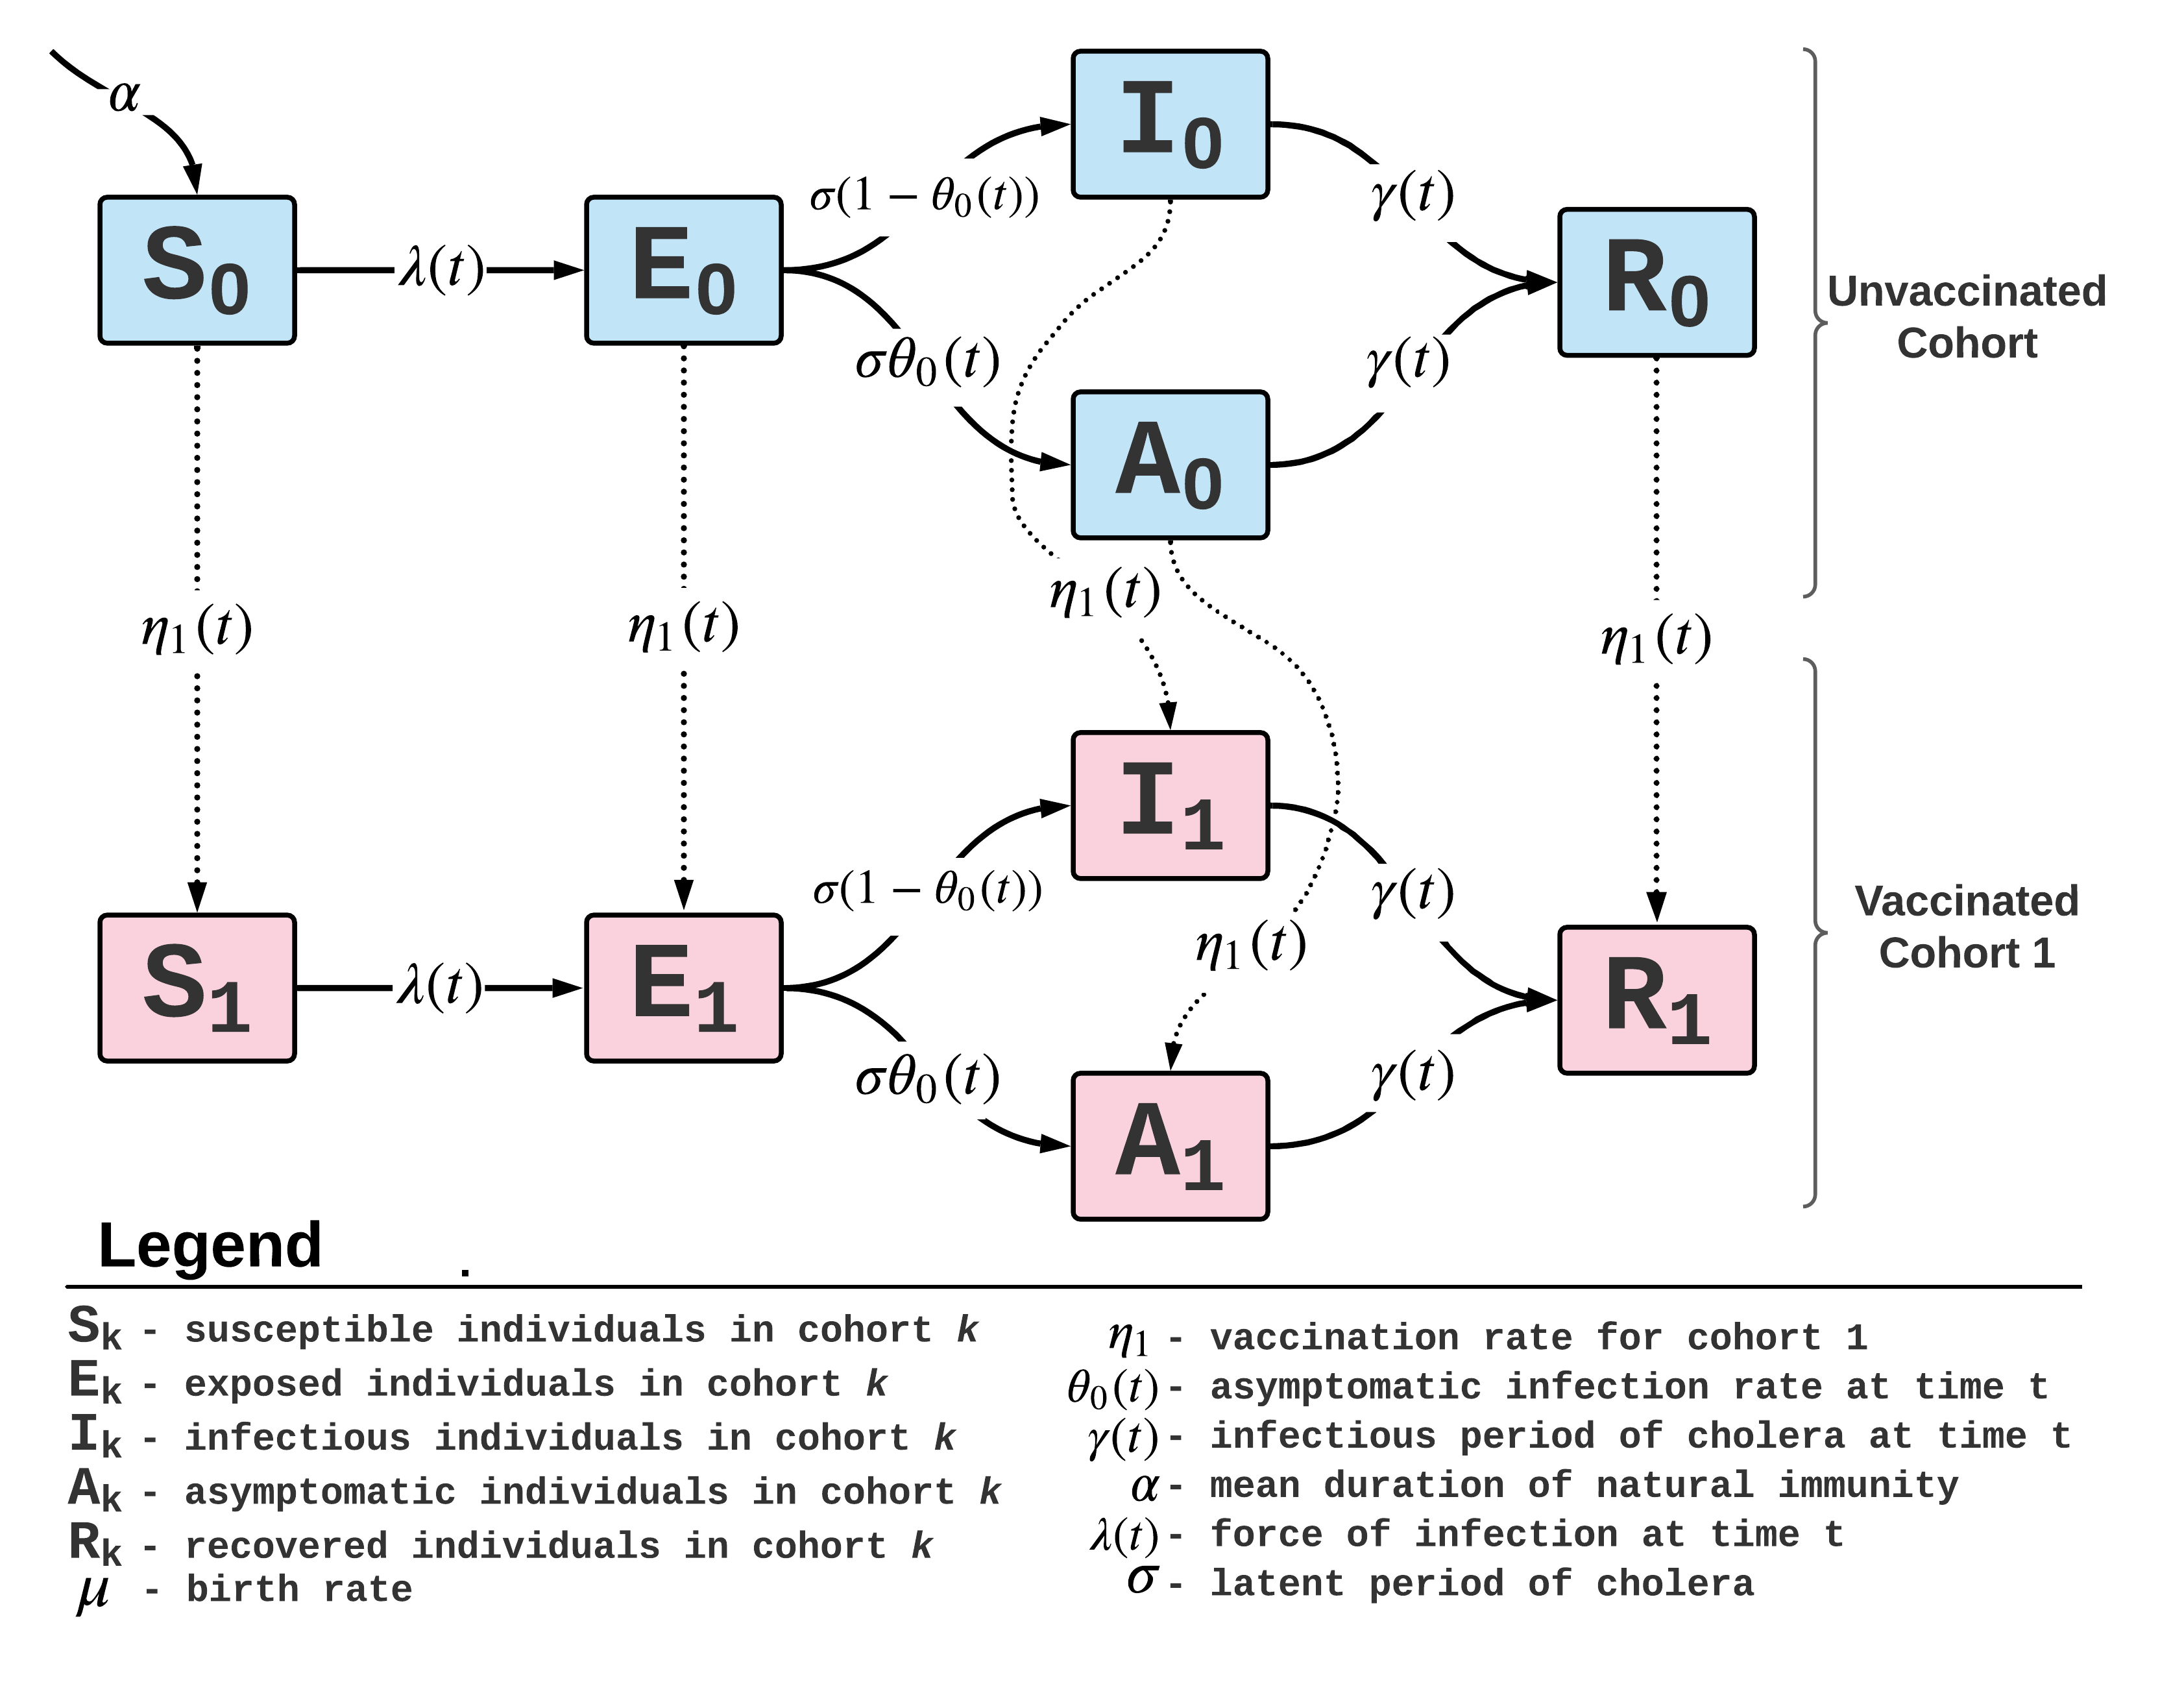
\includegraphics[width=170mm]{SEIAR.png}
          \caption{SEIAR compartment model diagram with one vaccination cohort adapted from Lee et al. \cite{Lee_supp}.}
        \end{figure}

\subsection{Reproduction}

 The preference for complex over simple models has been growing for several decades despite the fact that it has been shown that complexity is associated with decreases in forecasting accuracy \cite{Green}. Because epidemiological modelling is motivated by the need to accurately forecast disease prevalence to inform policy, we first establish a point of comparison for the evaluation of our model fit and quality. We elect to use a linear, Gaussian autoregressive moving average (ARMA) model of order (2,1) as it is a fairly simple model in which the current state depends only on previous states and white noise \cite{Shumway_ch3}. We can then compare the likelihood of the data under this model to the likelihoods achieved under our proposed models to evaluate whether the additional complexity is truly beneficial.
  
  Lee et al. divided the case data into two periods: epidemic (October 23rd, 2010 through March 31st, 2015) and endemic (April 1st, 2015 through January 12th, 2019) \cite{Lee_supp}. We adopted this breakpoint in our analyses. The ARMA(2,1) benchmark model achieved log-likelihoods of -1616.678, -1139.238, and -2800.808 for the epidemic, endemic, and the combined time period, respectively.
  
 After establishing benchmark log-likelihoods, we attempted to reproduce the results of Lee et al. as closely as possible in order to facilitate the evaluation of their model and parameter estimates. Lee et al. implemented their model in the R package \texttt{pomp} v1.19 and started the model calibration by generating 300 different sets of starting parameter values. They then used trajectory matching followed by iterated filtering to find a maximum likelihood estimate for the parameter values using each of the 300 sets. From the epidemic calibration, they pruned away sets resulting in filtering failures or extreme outlying values. The remaining sets were used as starting values for the endemic calibration in which all parameters were reestimated, excluding the initial state values ($E_0$ and $I_0$) \cite{Lee_supp}.

  We repeated most of this process with some minor changes. We did not perform trajectory matching as it assumes a deterministic latent process, which is not assumed in the forecasting model. Additionally, Lee et al. did not publish their initial starting sets, so we created our own using the schema provided in their supplemental code. We left weeks with missing data as \texttt{NA} rather than \texttt{0} as the \texttt{pomp} package is capable of working with missing data. We also filtered out epidemic parameter sets with $\nu \leq 0.9$ and $\beta_1 \geq 100$ and endemic parameter sets with log-likelihoods of -3000 units or less to avoid outlying parameter values similar to Lee et al.'s pruning process. Our reproduction (\hyperref[fig:A1]{fig. A1}) does seem to visually match the results of Lee et al. in figure S7 of their supplement \cite{Lee_supp}. 

\section{Model and Method Adjustments}

 Lee et al. did not report parameter point estimates as part of their findings. Rather, they used a cloud of parameter values to repeatedly simulate reported cases and then summarized over these simulations when plotting. This provided a relatively good visual match to the observed reported cases, but a cloud of parameter sets is not entirely helpful for inference and prediction as there is no clear method by which to evaluate the model's performance. For this reason, we propose slight adjustments to the model and methods in order to more rigorously predict cholera elimination and vaccination campaign efficacy in Haiti.

  We first suggest alternative algorithmic parameters when estimating model parameter values with the end goal of identifying maximum likelihood estimates. We used the improved iterated filtering algorithm as implemented in the \texttt{pomp} function \texttt{mif2()}. We elected to use 5000 particles and iterated 100 times in order to reduce variability in the log-likelihood estimates and to avoid potential particle depletion. Moreover, we increased the random walk standard deviations and created a larger set of starting values for the parameters for our global search for the MLE. In the following sections, we describe the structural alterations we made to the model.

\subsection{Overdispersion}

 Creating an equidispersed model can have inappropriate implications on the biological processes assumed to be driving the model. Especially in the case of epidemiological model development for the purpose of forecasting, the importance of incorporating enough stochasticity to explain the collected data has previously been discussed \cite{Breto_timeseriesmech, King_av}. The model proposed by Lee et al. did take stochasticity into consideration by estimating $\tau$, the inverse dispersion parameter for the negative binomial distribution simulator used in the measurement process \cite{King_statinfpomp, Lee_supp}.
        \begin{equation}
        \mathcal{C}_t = \textrm{NegBinom}(\rho \xi, \tau); \hspace{10mm} \mathcal{C}_t = \textrm{cases at time } t, \hspace{1mm} \rho = \textrm{force of infection}, \hspace{1mm} \xi = \textrm{incidence}
        \end{equation}
\noindent However, their latent process remained equidispersed. Calibrations to the epidemic period achieved log-likelihoods of no greater than -1823.403 units, and calibrations to the endemic period only -1143.416. Though their model's log-likelihood was greater than that of the ARMA benchmark model in the endemic period, their model was not competitive in the epidemic period as it achieved a log-likelihood over 200 units below the ARMA model's. In an attempt to achieve higher likelihoods in the epidemic period, we included the addition of another parameter, $\sigma^2$, the variance of a gamma white noise process that provided a multiplicative effect upon the force of infection:
        \begin{equation}
        \omega \sim \mathrm{Gamma}(\sigma^2, dt); \hspace{5mm}
        \lambda(t) = \frac{(I(t) + (1 - \kappa)A(t))^{\nu}\beta}{N(t)} \times \frac{\omega}{dt}
        \end{equation}
\noindent where $dt$ is the time interval, $\lambda(t)$ is the force of infection at time $t$, $\kappa$ is the assumed reduction in infectiousness of asymptomatic individuals, $\nu$ is a population mixing coefficient, $I(t)$ is the proportion of the population that is infectious at time $t$, $A(t)$ is the proportion of the population that is asymptomatic at time $t$, and $N(t)$ is the total population of Haiti at time $t$.

\subsection{Model Fitting}

 Using the maximum likelihood estimates of the parameters from this adjusted model's calibration, we plotted the simulated case reports against the case data (\hyperref[fig:2]{fig. 2}). Using point estimates has the added advantage of facilitating model evaluation and interpretability. For example, having a single value for the reporting rate, $\rho$, rather than a range enables us to calculate a single likelihood value for model comparison and provides more specific information about the disease's progression through the population. 
        \begin{figure}[H]
          \centering
          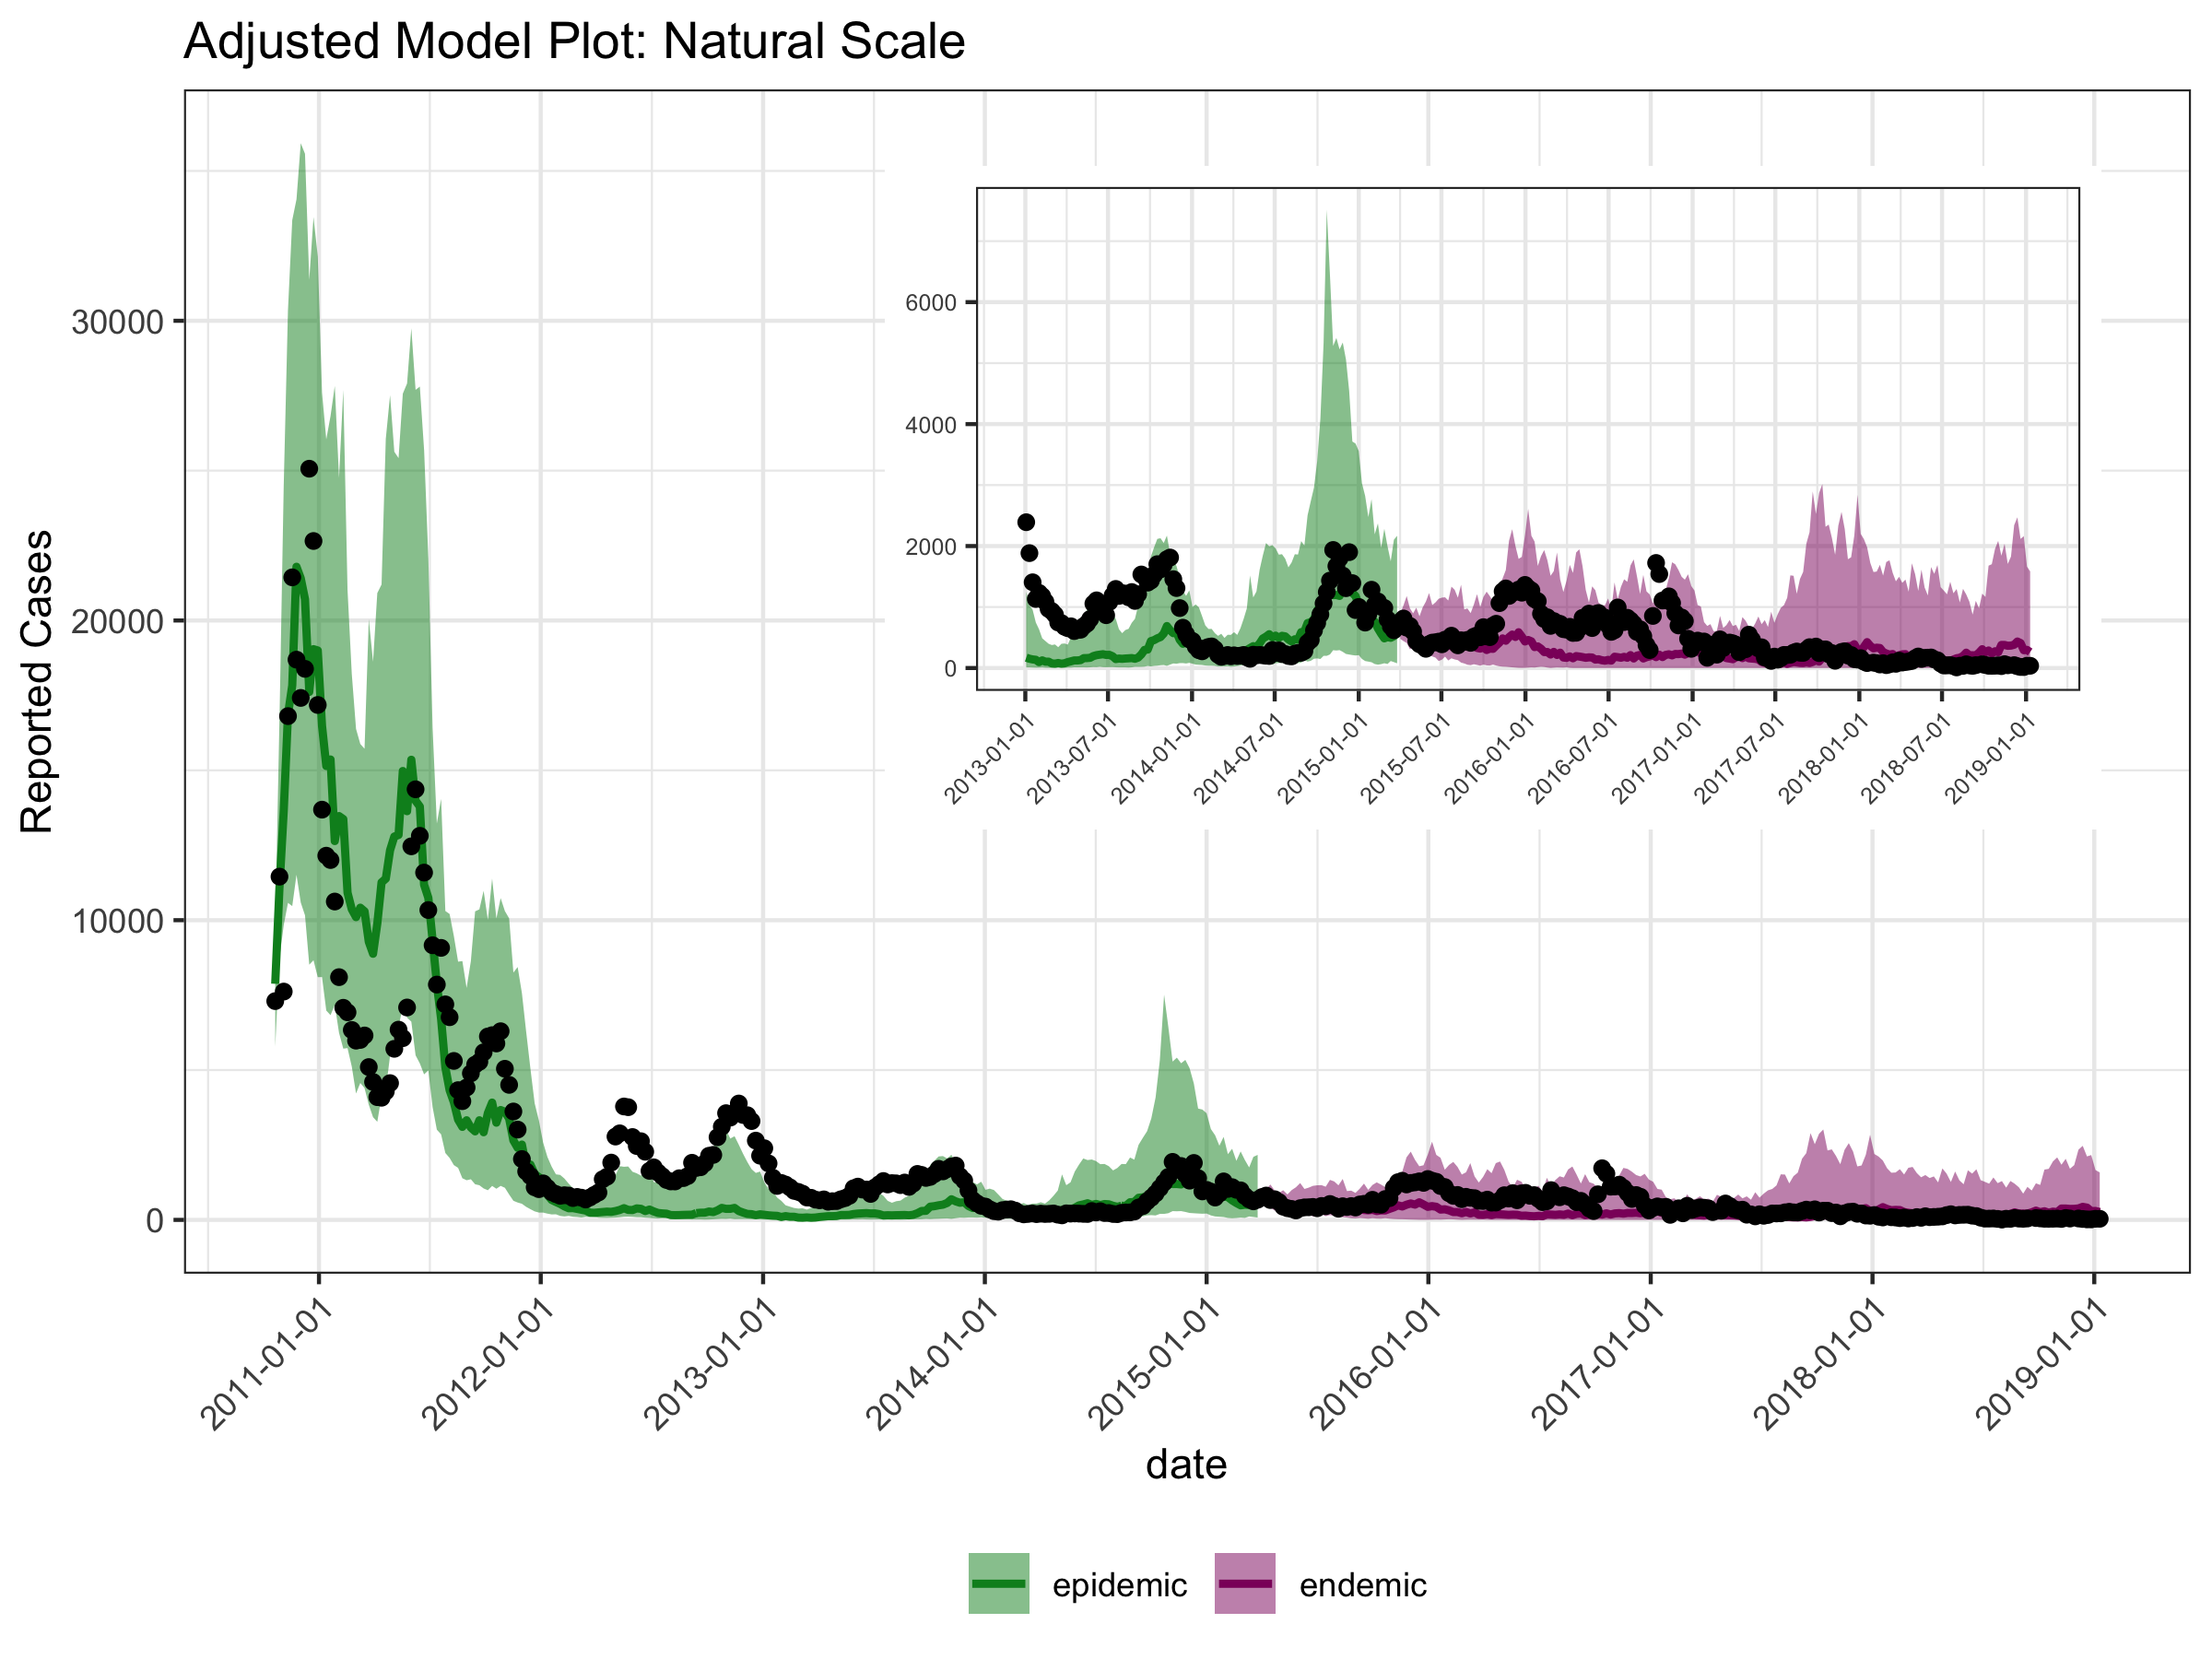
\includegraphics[width=150mm]{adj_inset.png}
          \caption{Plot of model simulations with overdispersion in the latent process using the parameter MLEs. Solid line indicates the median simulated reported cases across parameter sets. Ribbon indicates the 2.5th and 97.5th percentiles for the simulated reported cases. Inset provides a closer view of the model fit from 2013 through 2018.}
          \label{fig:2}
        \end{figure}

\subsection{Profile Likelihood}

 It is less than ideal to evaluate model fit or perform model selection using solely visual convergence of simulations. Because of this, we reestimated all parameters with the exception of $\sigma^2$ to create a profile log-likelihood plot over $\sigma^2$ and get a better idea of the MLE for this parameter.
        \begin{figure}[H]
          \centering
          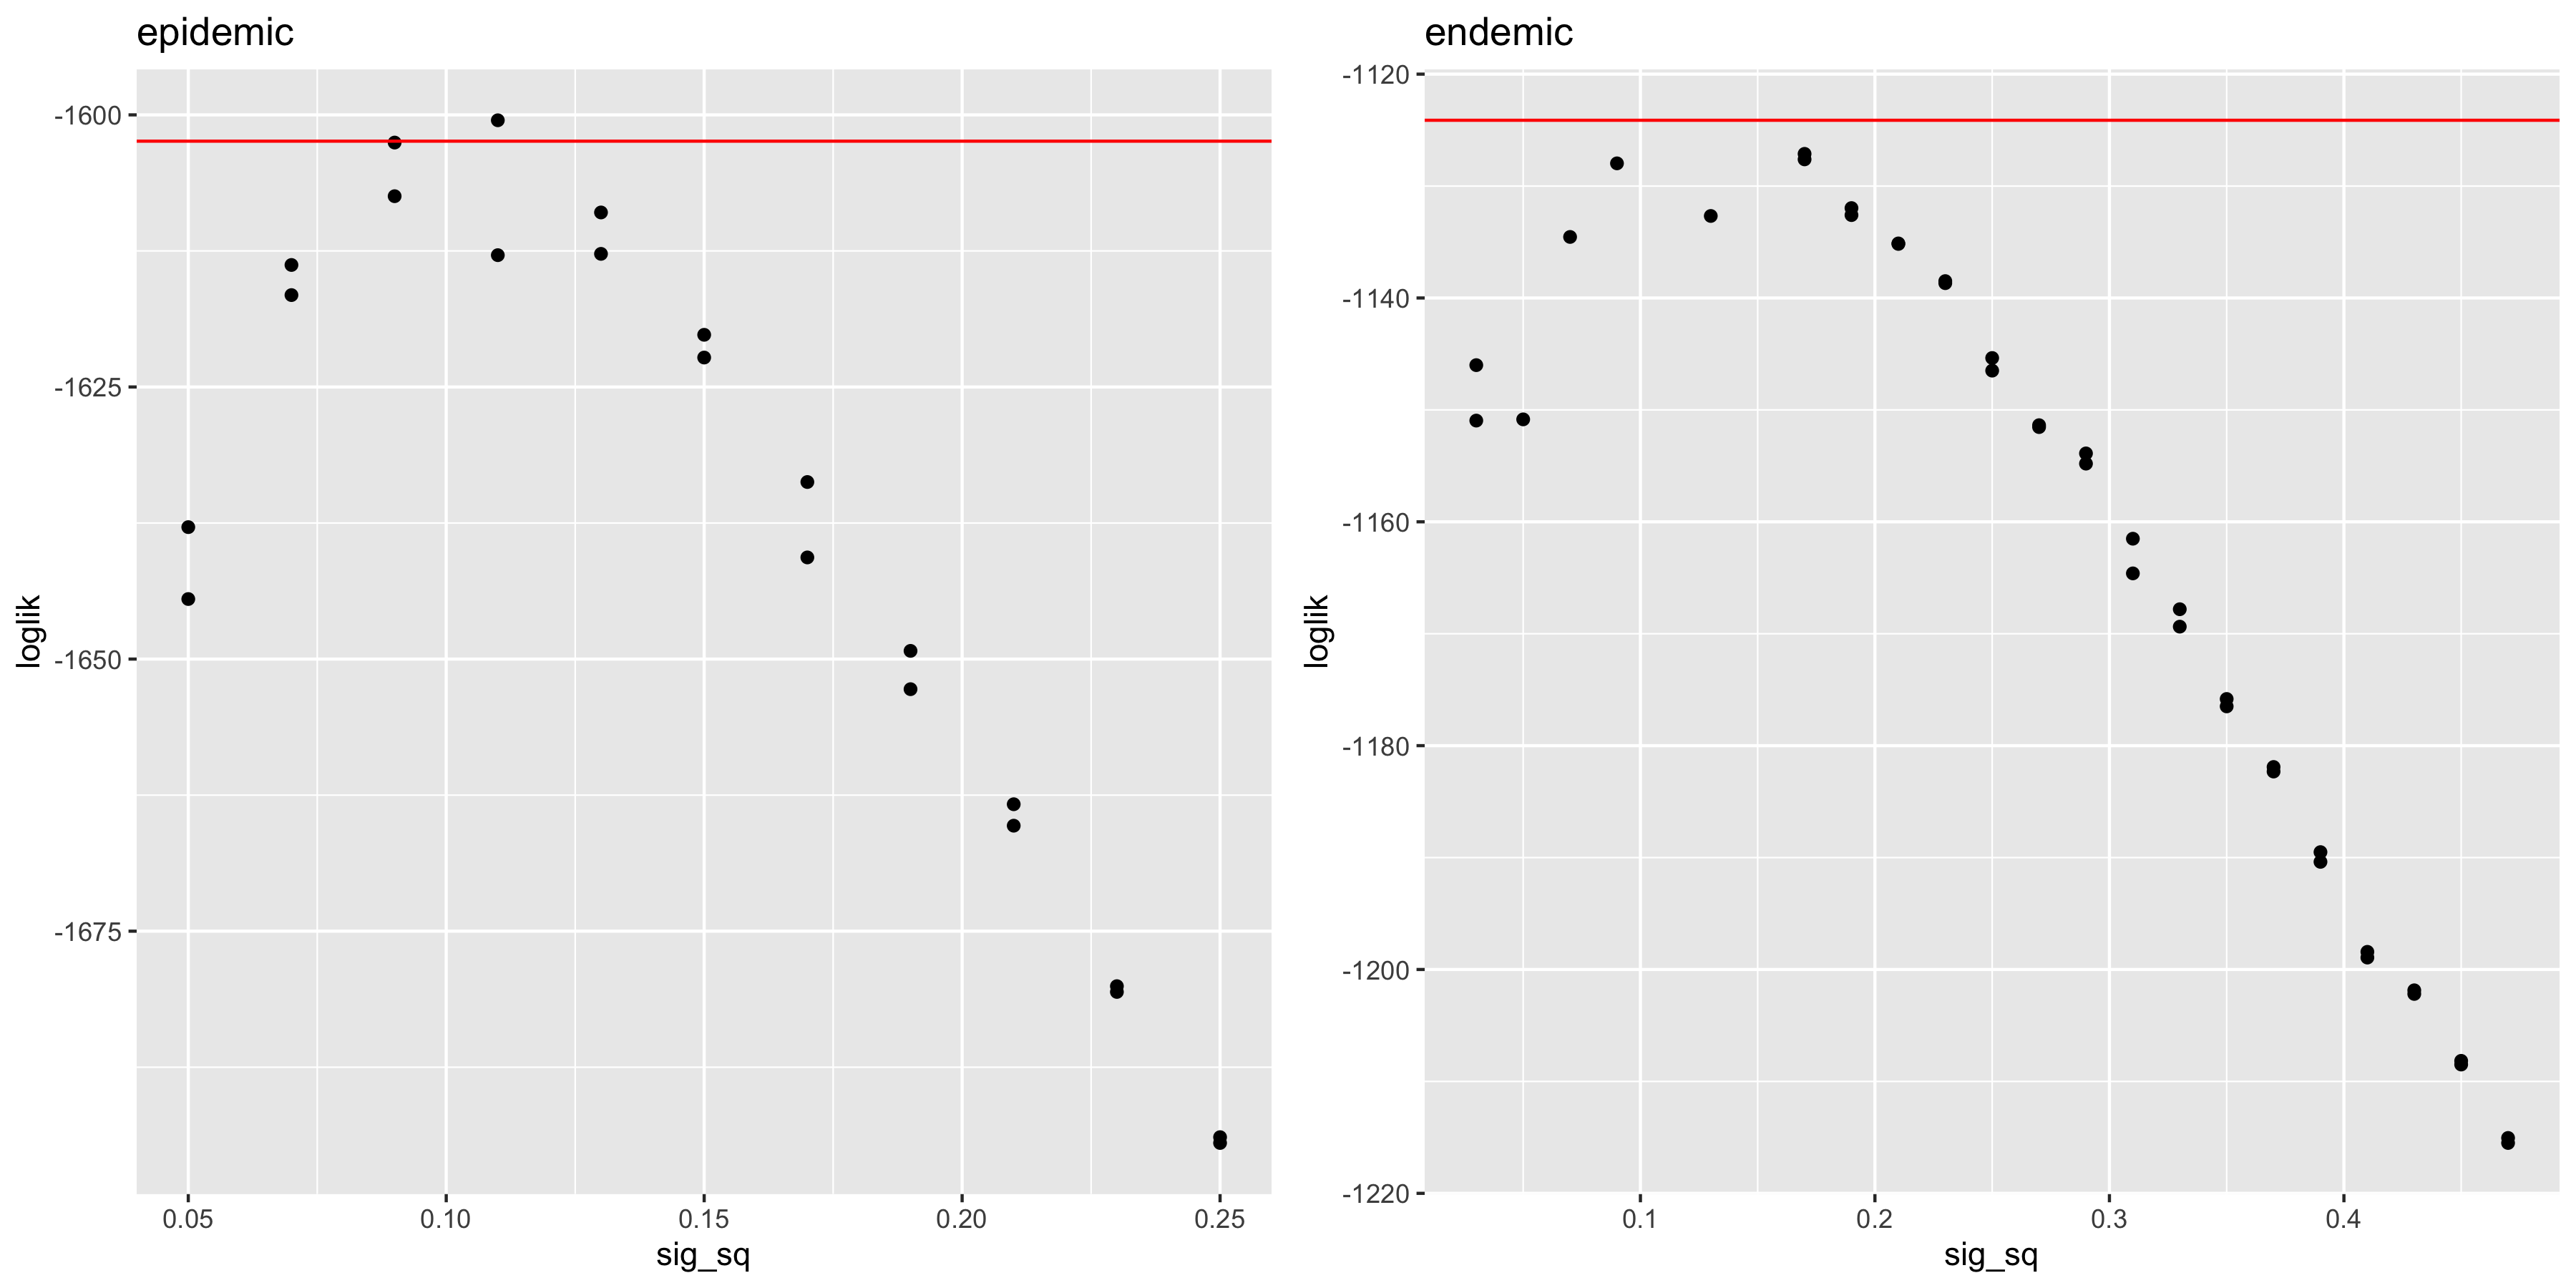
\includegraphics[width=150mm]{prof_lik_plot.png}
          \caption{Profile log-likelihood plot over $\sigma^2$ for the epidemic and endemic periods. The locations at which the red line intersects the curve connecting the points (not pictured) indicate the 95\% confidence interval for $\sigma^2$.}
          \label{fig:3}
        \end{figure}

  From this figure, we see that $\sigma^2$ values of around 0.09 to 0.13 in the epidemic period and 0.09 to 0.16 in the endemic period are most consistent with the case data and have associated log-likelihoods in the epidemic and endemic periods of upwards of -1610 and -1130, respectively. This profile log-likelihood plot provides a better understanding of the amount of uncertainty accompanying our estimate of $\sigma^2$ \cite{Cole}. The narrow confidence interval, lack of identifiability issues, and improvement in log-likelihood support the inclusion of this parameter in the model. 

\subsection{Joint Estimation}

  Lee et al. proceeded by fitting the model to the epidemic period, simulating to the end of the epidemic period with each set of parameter estimates, and then they used the final states to reestimate all of the parameters for the endemic period. Though this method did achieve relatively good looking simulations with reasonably high log-likelihoods after adding $\sigma^2$, there is justification for linking the two estimation procedures more closely. For one, it is mechanistically logical to use all of the available data to inform the estimation of parameters that are present in the model during both periods. As the designation of the break-point between periods is somewhat arbitrary and the epidemiological system exists without respect for this breakpoint, it also may be better to estimate demographic and seasonal parameters without respect for this break-point.
  
  We fit the model to the epidemic and endemic periods simultaneously, estimating only $\rho$, $\tau$, and $\sigma^2$ separately. This jointly estimated model performed quite well with a log-likelihood of about -2734.761, beating the ARMA benchmark by over 50 log-likelihood units.
        \begin{figure}[H]
          \centering
          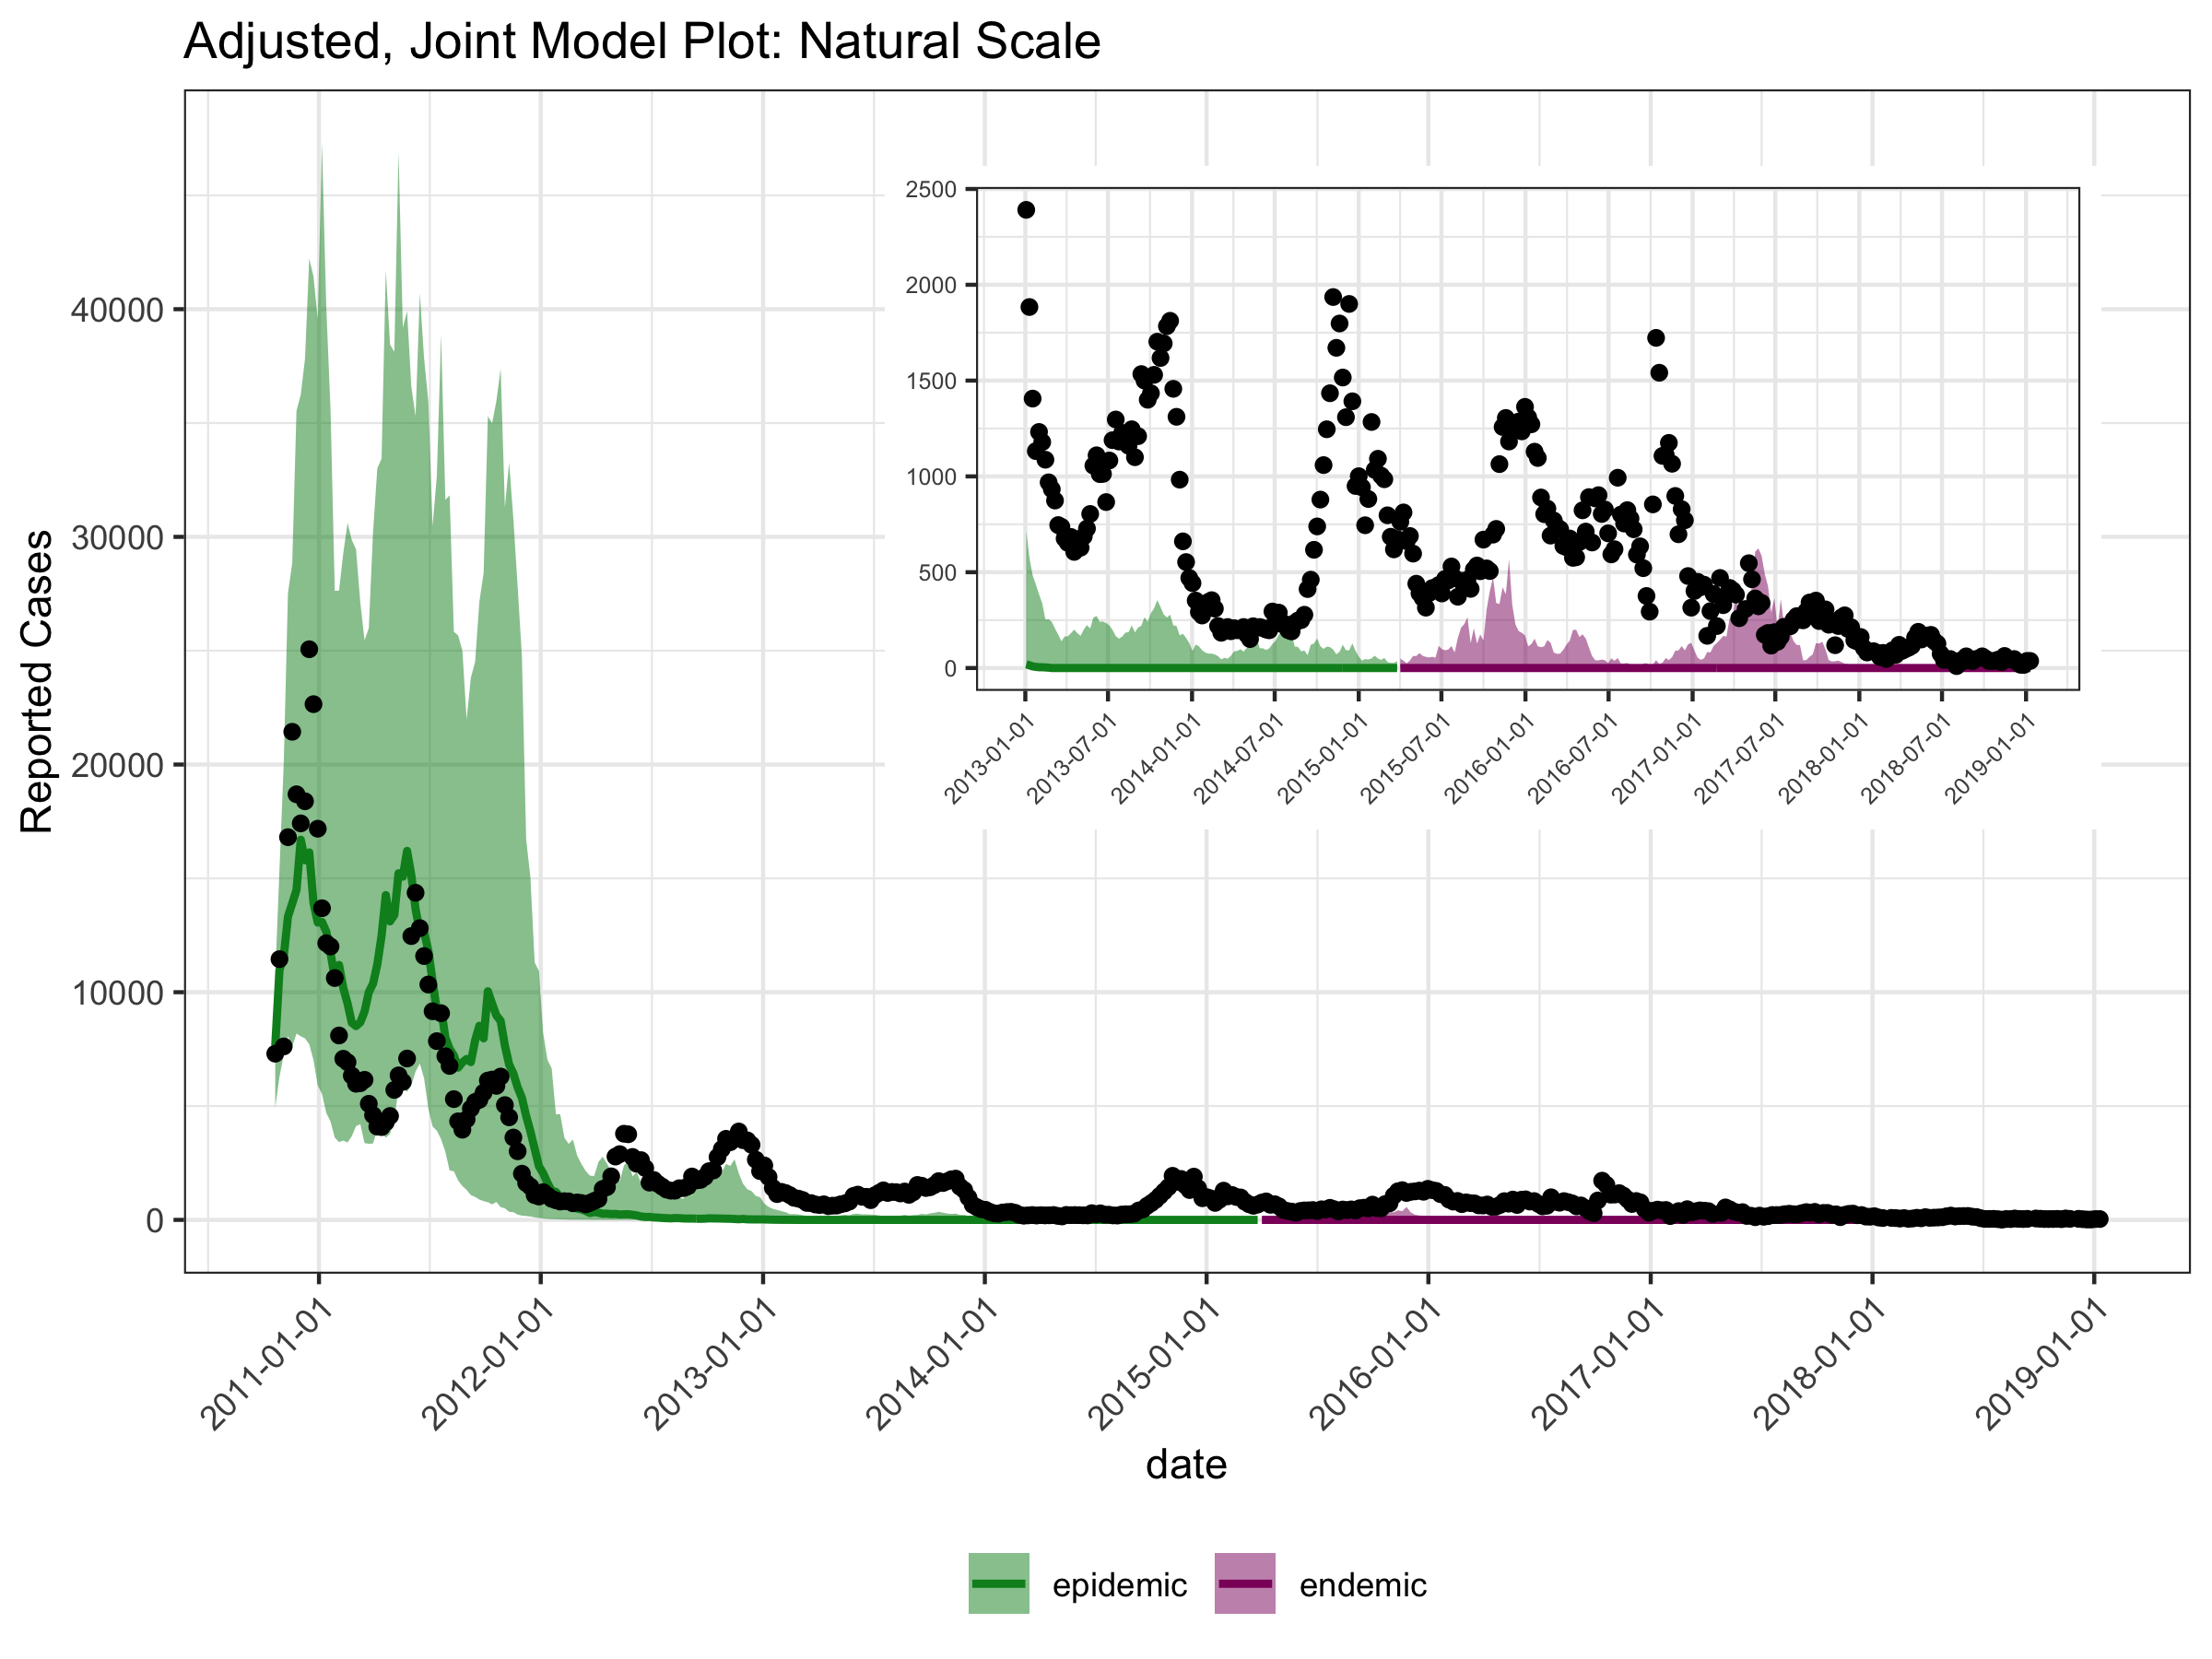
\includegraphics[width=150mm]{joint_inset.png}
          \caption{Plot of simulations from the jointly estimated model with additional overdispersion in the latent process using the maximum likelihood estimates of the model parameters. Solid line indicates the median number of reported cases from simulations. Ribbon indicates the 2.5th and 97.5th percentiles for the simulated reported cases. Inset provides a closer view of the model fit from 2013 through 2018.}
          \label{fig:4}
        \end{figure}

\subsection{Model Comparison}

 Though these models are all closely related, they are not nested and so we cannot select a model based upon a likelihood ratio test. However, a comparison of likelihoods is still informative so long as we keep in mind the nature of the models' relationship. The Akaike Information Criterion (AIC) is a likelihood-based measure that can be used for model selection that applies a penalty to a model's score according to its complexity. Below we supply an AIC table (\hyperref[tab:1]{table 1}) for comparison of the four models discussed above: the ARMA(2, 1) benchmark model, the original model proposed by Lee et al., the altered model with latent process noise, and the jointly estimated altered model. 

  We estimated the log-likelihoods for the two altered models using repeated particle filters and the parameter maximum likelihood estimates. For Lee et al.'s original model, we report the best possible likelihood achieved across all calibration parameter sets. The full log-likelihoods were calculated as the sum of the likelihoods from the epidemic and endemic periods for the models without joint estimation. The joint model log-likelihoods for the epidemic and endemic periods were calculated as the sum of the conditional log-likelihoods at each time point in the corresponding time periods. We took the average of 20 replications of the particle filter. 
        \begin{table}[H]
        \caption{Table of log-likelihoods by period, number of estimated parameters, and AIC are reported for the ARMA(2,1) benchmark model, original Lee et al. model, the altered model, and the jointly estimated altered model.}
        \label{tab:1}
        \begin{center}
        \begin{tabular}{||c | c c c c||}
         \hline
         Measure & ARMA Model & Lee et al. Model & Alt. Model & Joint Model \\ [0.5ex]
         \hline\hline
         Epi. Log-Lik. & -1616.678 & -1823.403 & -1600.133 & 1612.962 \\
         \hline
         End. Log-Lik. & -1139.238 & -1143.416 & -1121.02 & -1127.888 \\
         \hline
         Full Log-Lik. & -2800.808 & -2966.819 & -2721.153 & -2735.623 \\
         \hline
         Num. of Params. & 5 & 11+9=20 & 12+10=22 & 15 \\
         \hline
         AIC & 5611.616 & 5973.638 & 5486.306 & 5499.522 \\
         \hline
        \end{tabular}
        \end{center}
        \end{table}
        
  According to AIC, the altered model with the lowest score is the ideal model; however, bearing in mind the limitations of likelihood-based model selection discussed above, we opt to use the jointly estimated altered model in the following forecasting section. This decision was made based upon the model's greater log-likelihood compared to the original model as well as its lower complexity compared to the altered model without joint fitting. 

\section{Forecasting}

 The impetus behind many epidemiological modelling studies is the need to predict future outbreaks of a disease in order to avert widespread infection and death. For this reason, our final section concerns model forecasting with respect to the variety of vaccination campaigns studied by Lee et al. We used the jointly estimated altered model for our forecasting and did so for the following 6 scenarios:
        \begin{itemize}
        \item No Vaccinations
        \item Two Department: vaccination carried out in the Artibonite and Centre departments over two years
        \item Three Department: vaccination carried out in the Artibonite, Centre, and Ouest departments over 2 years
        \item Slow National: vaccination carried out in all 10 departments over 5 years
        \item Fast National: vaccination carried out in all 10 departments over 2 years
        \item Fast National, High-Coverage: vaccination carried out in all 10 departments over 2 years
        \end{itemize}
        
\noindent The first four vaccination campaigns assumed target population coverage of 70\% with two doses, 10\% with one dose, and 20\% with zero doses, while the Fast National, High-Coverage scenario assumed 95\%, 1.67\%, and 3.33\% for two-dose, one-dose, and zero-dose coverage, respectively. All vaccination efficacy and roll-out specifications were kept the same as in Lee et al. \cite{Lee_supp}.

  A simulation was said to achieve cholera elimination if its true incidence fell below one case for at least fifty-two consecutive weeks after the beginning of the vaccination campaign and remained below one case for the rest of the ten-year forecasting period. A simulation was said to achieve cholera elimination at $x$ years if the fifty-two consecutive week period began before the end of year $x$. Below we provide a table of the predicted probabilities of elimination of cholera after five years in all six scenarios for our jointly estimated altered model along with the probabilities found using the original model as reported by Lee et al. \cite{Lee_supp}. The probability of elimination was calculated as the proportion of simulations achieving five-year elimination. One thousand simulations were carried out for the joint model, but the number of simulations was not reported for the original model as it used a collection of parameter sets rather than repeated simulations with the parameter MLEs.
        \begin{table}[H]
        \caption{Table of estimated probabilities of elimination of cholera by vaccination scenario for the original Lee et al. model and the jointly estimated, altered model \cite{Lee_supp}.}
        \begin{center}
        \begin{tabular}{||c | c c c c c c ||}
         \hline
         Model & No Vac. & 2-Dept. & 3-Dept. & Slow Nat. & Fast Nat. & Fast Nat., High Cov. \\ [0.5ex]
         \hline\hline
         Original & 5.8\% & 32.7\% & 64.5\% & 71.6\% & 79.6\% & 88.2\% \\
         \hline
         Altered & 99.0\% & 100\% & 100\% & 100\% & 100\% & 100\% \\
         \hline
        \end{tabular}
        \end{center}
        \end{table}
        
  The jointly estimated altered model predicted the elimination of cholera in all scenarios with very high probability. Plots of the simulated reported cases and true incidence by vaccination scenario (\hyperref[fig:A2]{fig. A2}, \hyperref[fig. A3]{fig. A3}) show that the elimination time was reduced as vaccination administration grew more rigorous. Interestingly, even in the case of no intervention, the model predicted fade-out of the disease by the start of 2021. These results contrast with the forecasting conducted by Lee et al. which predicted seasonal variation in the number of cases (zero to upwards of two thousand cases) across all scenarios as well as very low probability of elimination in the No Vaccination scenario with the possibility of reemergence \cite{Lee_supp}.

\section{Discussion}

 Using a combination of Monte Carlo, maximum likelihood, and simulation-based methods, we evaluated a stochastic state\hyp{}space model for the 2010-2011 Haiti cholera epidemic proposed by Lee et al. at the Bloomberg School of Public Health along with two of our own variations on the model \cite{Lee_haiticholera}. Though only consisting of minor adjustments in the calibration methodology and latent process specification, these altered models achieved improvements in likelihood over the original model.

  These varied likelihood estimates coupled with the differences in forecasting results emphasize the importance of rigorous model fitting and interrogation. Epidemiological models can be of great importance when faced with an infectious disease outbreak as they can provide insights into the potential effectiveness or failure of intervention plans to mitigate spread. However, the utility of these models hinges upon the assumption that they are appropriate for the situation; that is, that they are able to come close to describing the data-generating process(es). Whether due to improper parameter estimation or model misspecification, a model that is unable to explain the data is not likely to produce accurate predictions and is ultimately of little use to researchers and public health officials alike.
   
\subsection{Limitations}

 After the onset of the epidemic, the Haiti Ministry of Health and Population began a national plan for combating cholera. The plan included an assortment of interventions including improvements to sanitation, water accessibility, and strict case monitoring \cite{tohme}. Because of the time needed to implement large-scale changes to the water infrastructure of the country, many small vaccination campaigns were carried out from 2012 to 2018 as a first step to mitigating the spread. The number of individuals receiving at least one dose totaled over 1.5 million, or approximately 9\% of the population of Haiti. Case-area targeted interventions (CATIs) consisting of cholera education, disinfecting spray, soap, and chlorine tablets were also supplied to over 48,000 locations across the country \cite{Rebaudet}.
  
   In this case study, the data used to fit all the models included 430 weeks of case data spanning October 23rd, 2010 through January 12th, 2019. This interval overlaps significantly with the periods in which the series of vaccination campaigns and CATIs were deployed. However, none of these models included mechanisms for the campaigns or the intervention programs. As a consequence of this, we remain critical of the final model parameter estimates reported in \hyperref[tab:A1]{table A1} despite the fact that our adjusted models are competitive with the simple ARMA model. Maximum likelihood estimation attempts to find the parameter values for a model that maximize the probability of observing the data. This can come with unintended consequences related to the mechanisms underlying the processes of interest. There is the possibility that the MLE we found for any given parameter is not a good estimate of the true parameter value as the MLE may be biologically or ecologically improbable. In addition, the model construction can greatly influence the parameter estimates. In the case of our study, the exclusion of the vaccination campaigns and intervention programs may have led to other parameters compensating for the omitted model components in order to explain the data. Although our altered models outperformed that of the original authors according to likelihood\hyp{}based measures, we must be mindful of the relationships between model construction, model fitting, and model quality.
   
   Looking more deeply at \hyperref[fig:2]{figure 2} and \hyperref[fig:3]{figure 3}, it is clear that the simulations do not match the case reports in the period after the start of 2013 as closely as in the years prior to this point. The discrepancy between the data and the model simulations is more clearly visible when plotting on the natural logarithmic scale as in \hyperref[fig:A4]{fig. A4}, \hyperref[fig:A5]{fig. A5}, \hyperref[fig:A6]{fig. A6}). To understand why the change of scale highlights this disparity, suppose we have a dataset of two measurements: 1 case in week one and 100 cases in week two. We simulate cases and get 6 cases in week one and 105 cases in week two. Plotting this on the natural scale would show the same relative difference of 5 cases between the simulations and measurements. However, in week one we overestimated the number of cases by a factor of 6, while in week two we only overestimated by a factor of 1.05. Transforming the cases with the natural logarithm allows us to better diagnose model problems by illustrating these differences in magnitude. 
   
   It is also important to note that there are many other methods of model criticism that can be carried out to even more thoroughly evaluate model quality and fit \cite{Millar, Cole}. Additional likelihood profiles and model diagnostics such as plots of the autocorrelation between cases at different time points as well as analysis of the spatial distribution of cases and the variability of case forecasts through time can be instrumental in assessing a model's appropriateness in context \cite{King_av}. Due to the nature of maximum likelihood estimation and the iterated filtering algorithm, there is also the option to carry out a more exhaustive search throughout the parameter space when fitting the model. The algorithmic parameters of IF2 include starting values for all estimated parameters, the number of particles used when filtering, and the number of iterations \cite{Ionides_infpomp}. In an attempt to balance the price of computation with rigor of results, we used 500 sets of starting values, 5000 particles, and 200 iterations when fitting the adjusted models. But by using a larger number of starting points, particles, and iterations, one might be able to identify parameter values that achieve a higher likelihood. 
   
   Despite the fact that our models failed to produce simulations that visually matched the case data, we maintain that our study was successful. We aimed to exhibit crucial steps in epidemiological model construction and application by building upon the framework established by Lee et al. \cite{Lee_haiticholera}. We therefore restricted our adjustments of the original model to minor alterations in order to underscore this important relationship between model development and model quality. Though the poorly matching simulations indicate that additional improvements can be made, the greater likelihoods and vastly contrasting forecasts still illustrate the significance of thorough model fitting procedures and proper model specification.

\section{Conclusion}

 There have been no laboratory confirmed cases of or deaths caused by cholera in Haiti since early 2019, most likely due to the fast and widespread deployment of CATIs because of the limited distribution of vaccinations \cite{Rebaudet}. Similar to the reality of the last few years and Haiti's response to the epidemic, our jointly estimated altered model predicted the natural elimination of cholera by early 2021 without any vaccination interventions. Though conducted post hoc, these results have promising implications for the model's quality and, more broadly, for the application of mathematical modelling for disease transmission to informing public health decision-making.

  Many of the techniques and methods used in this demonstration of the power of simulation\hyp{}based inference can be extended to current and future epidemiological contexts such as the recent magnitude 7.2 earthquake that hit Haiti in August of 2021. Over 1,800 water supply systems, 53 healthcare sites, and 130,000 homes have been damaged by the earthquake and Tropical Depression Grace \cite{uni}. Though cholera has not been observed in Haiti for upwards of three years, the threat of its reemergence is present, especially considering the fact that the 2010-2011 epidemic arose in the aftermath of a magnitude 7.0 earthquake that ravaged the country and its infrastructure \cite{Sanon}. Hopefully, proper modelling can be helpful in informing policy by providing insights into the efficacy of potential response plans in an effort to avert a second cholera epidemic.

\newpage

\section{Appendix}

\renewcommand{\thefigure}{A\arabic{figure}}
\setcounter{figure}{0}
\renewcommand{\thetable}{A\arabic{table}}
\setcounter{table}{0}
\begin{table}[H]
\caption{Table of parameter values achieving the maximum likelihood for the epidemic (epi) and endemic (end) calibrations separately with the exception of the jointly estimated altered model in which the two periods were combined. Parameters reported include reporting rate ($\rho$), measurement process overdispersion ($\tau$), latent process overdispersion ($\sigma^2$), population mixing coefficient ($\nu$), and seasonality terms ($\beta_{1:6}$). All parameters are reported to 4 decimal places.}
\label{tab:A1}
\begin{center}
\begin{tabular}{||c | c c c c c ||}
 \hline
 Model & $\rho$ & $\tau$ & $\sigma^2$ & $\nu$ & $\beta_{1:6}$ \\ [0.5ex]
 \hline\hline
 Original (epi) & 0.8220 & 15.2111 & NA & 0.9811 & \makecell{3.0048, 3.8524,\\2.4215, 3.7633,\\3.2372, 3.4116}\\
 \hline
 Original (end) & 0.9968 & 22.2507 & NA & 0.9925 & \makecell{3.1299, 3.3738,\\2.1317, 3.3409,\\2.8502, 2.7652}\\
 \hline
 Altered (epi) & 0.3148 & 376.7802 & 0.1016 & 0.9841 & \makecell{5.3324, 2.6566,\\3.8325, 2.7666,\\5.0974, 1.8034}\\
 \hline
 Altered (end) & 0.9517 & 85.4460 & 0.01122 & 0.9869 & \makecell{2.4296, 4.1216,\\2.0811, 3.7738,\\2.4402, 3.6037}\\
 \hline
 Joint, Altered & \makecell{0.4765 (epi)\\0.4497 (end)} & \makecell{688.7796 (epi)\\105.3583(end)} & \makecell{0.1106 (epi)\\0.1677 (end)} & 0.9976 & \makecell{4.0148, 2.7089,\\2.7423, 3.0589,\\3.5747, 2.2309}\\
 \hline
\end{tabular}
\end{center}

\end{table}
\begin{figure}[H]
  \centering
  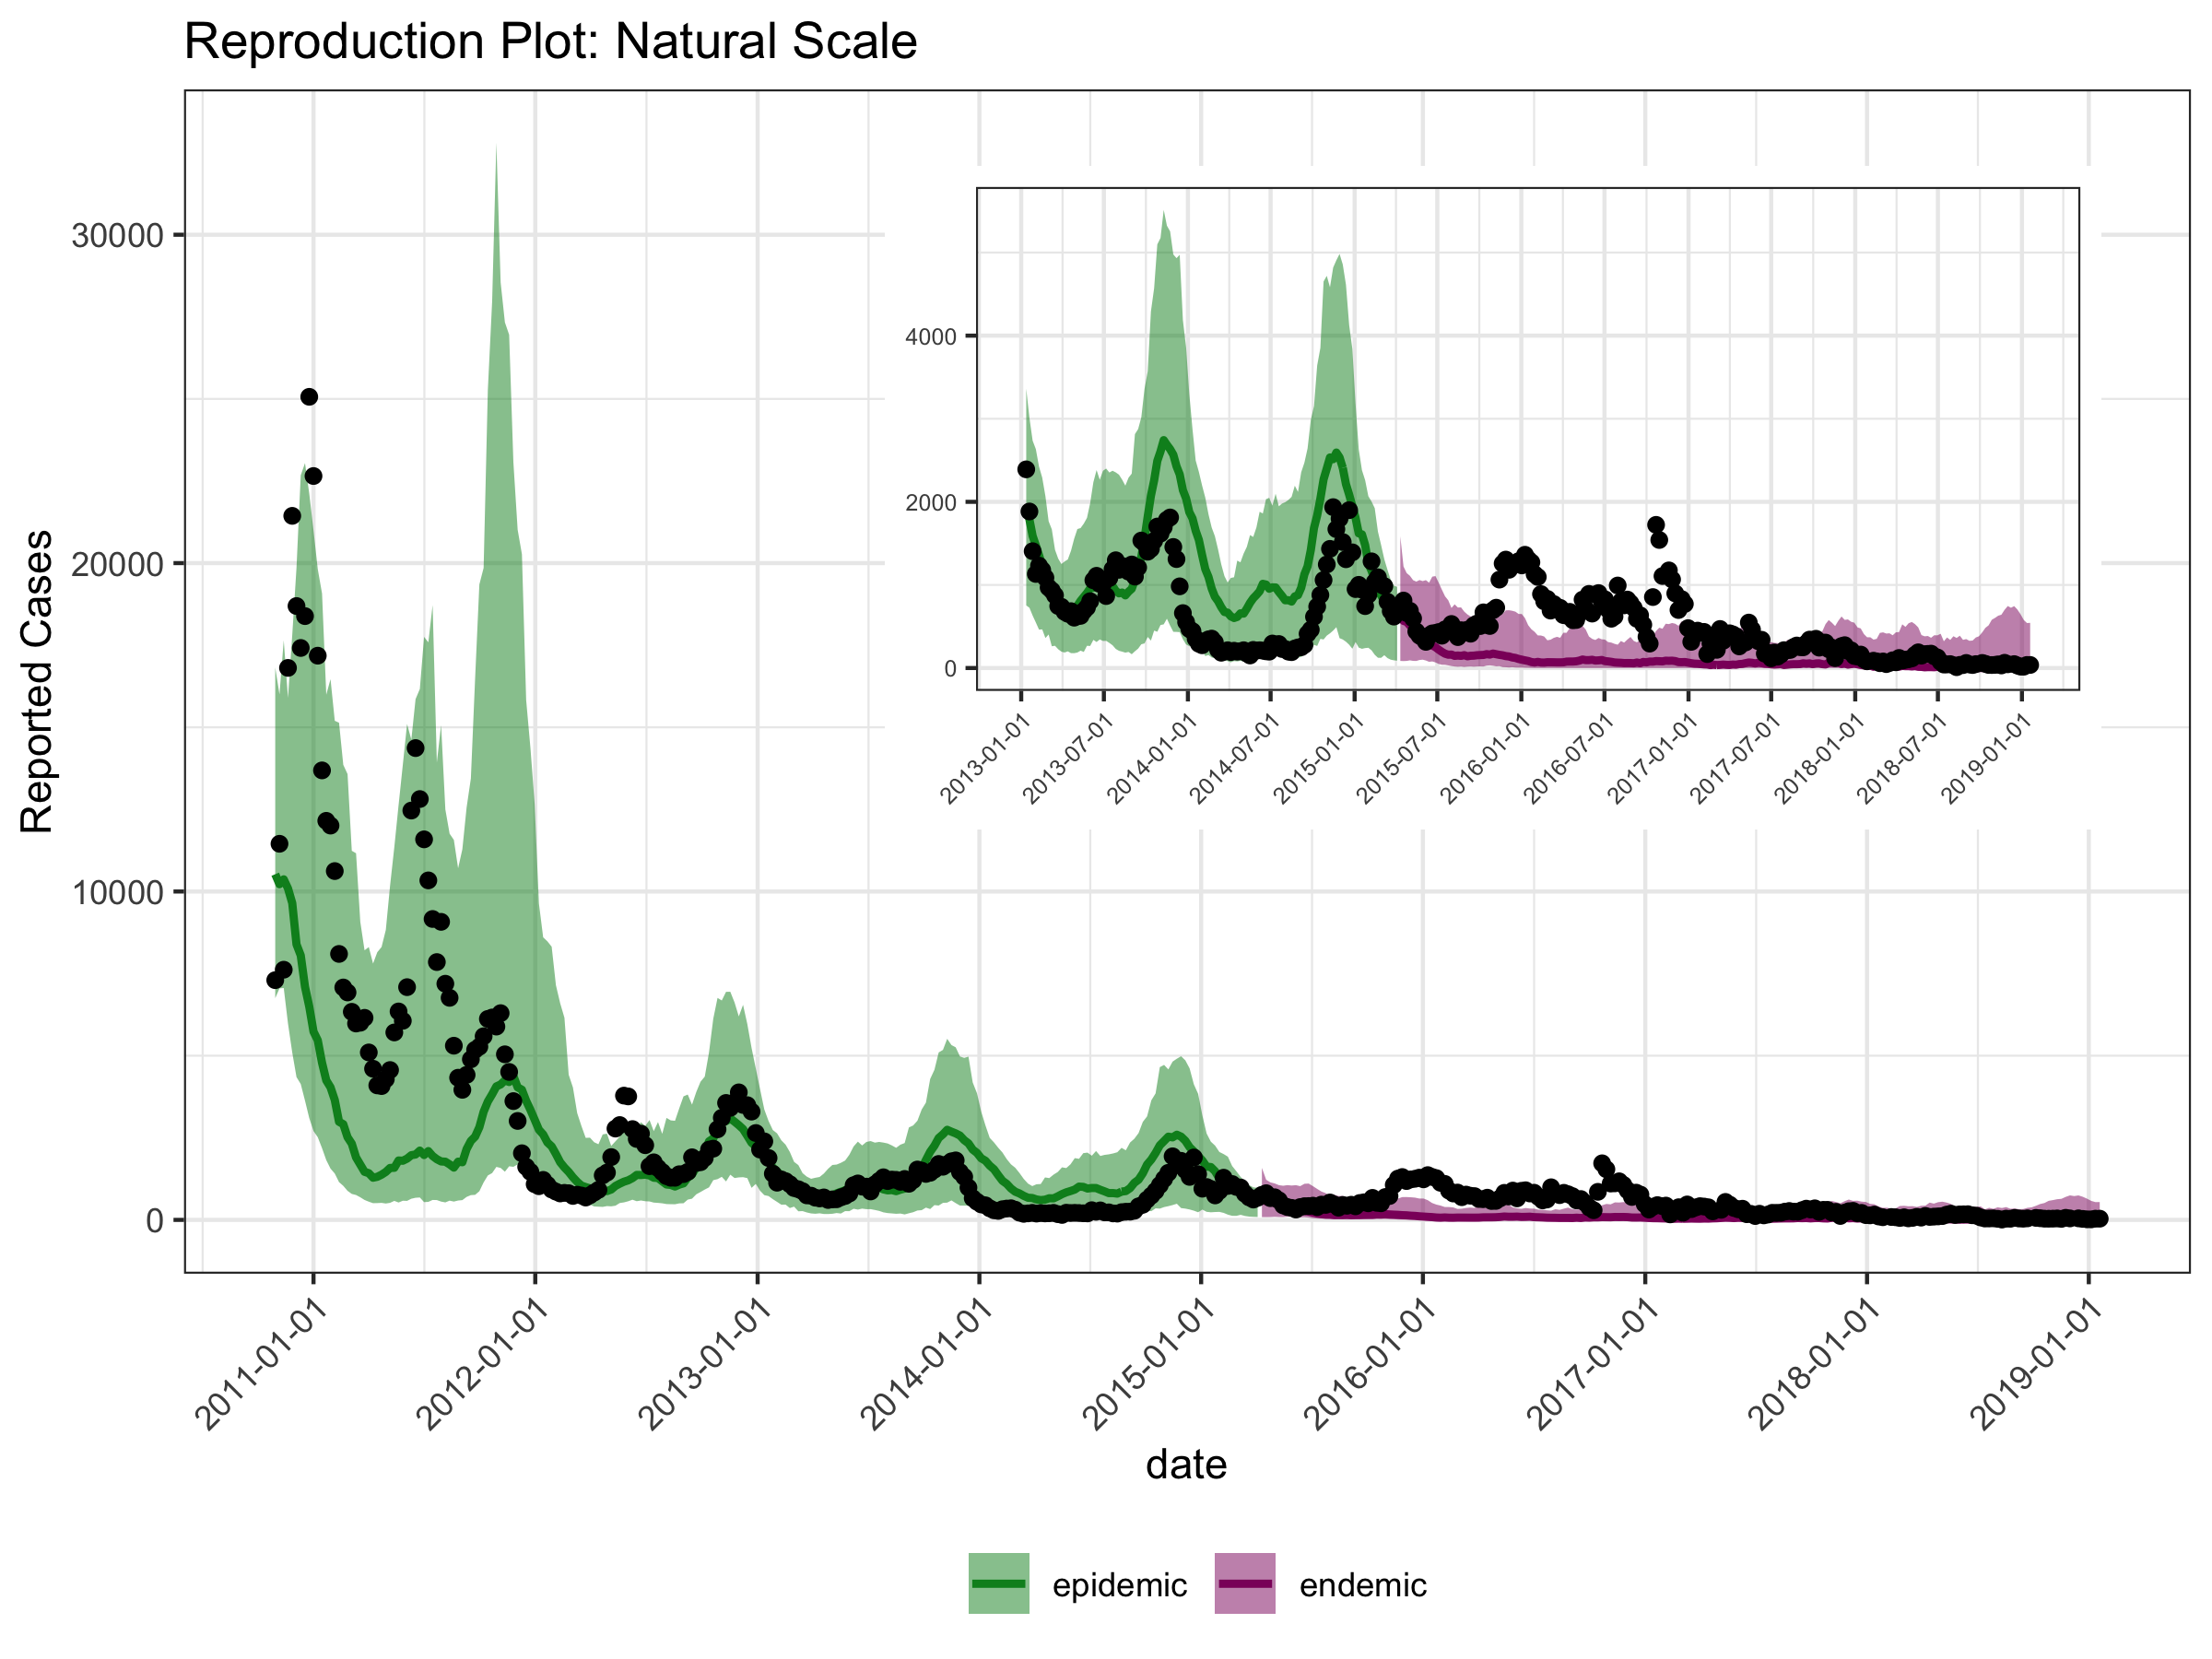
\includegraphics[width=150mm]{reprod_inset.png}
  \caption{A reproduction of figure S7 of Lee et al. \cite{Lee_supp}. The solid line indicates the median number of reported cases from the simulations across sets of parameters, and the ribbon indicates the 2.5th and 97.5th percentiles for the simulated reported cases. Inset provides a closer view of the model fit from 2013 through 2018.}
  \label{fig:A1}
\end{figure}

\begin{figure}[H]
  \centering
  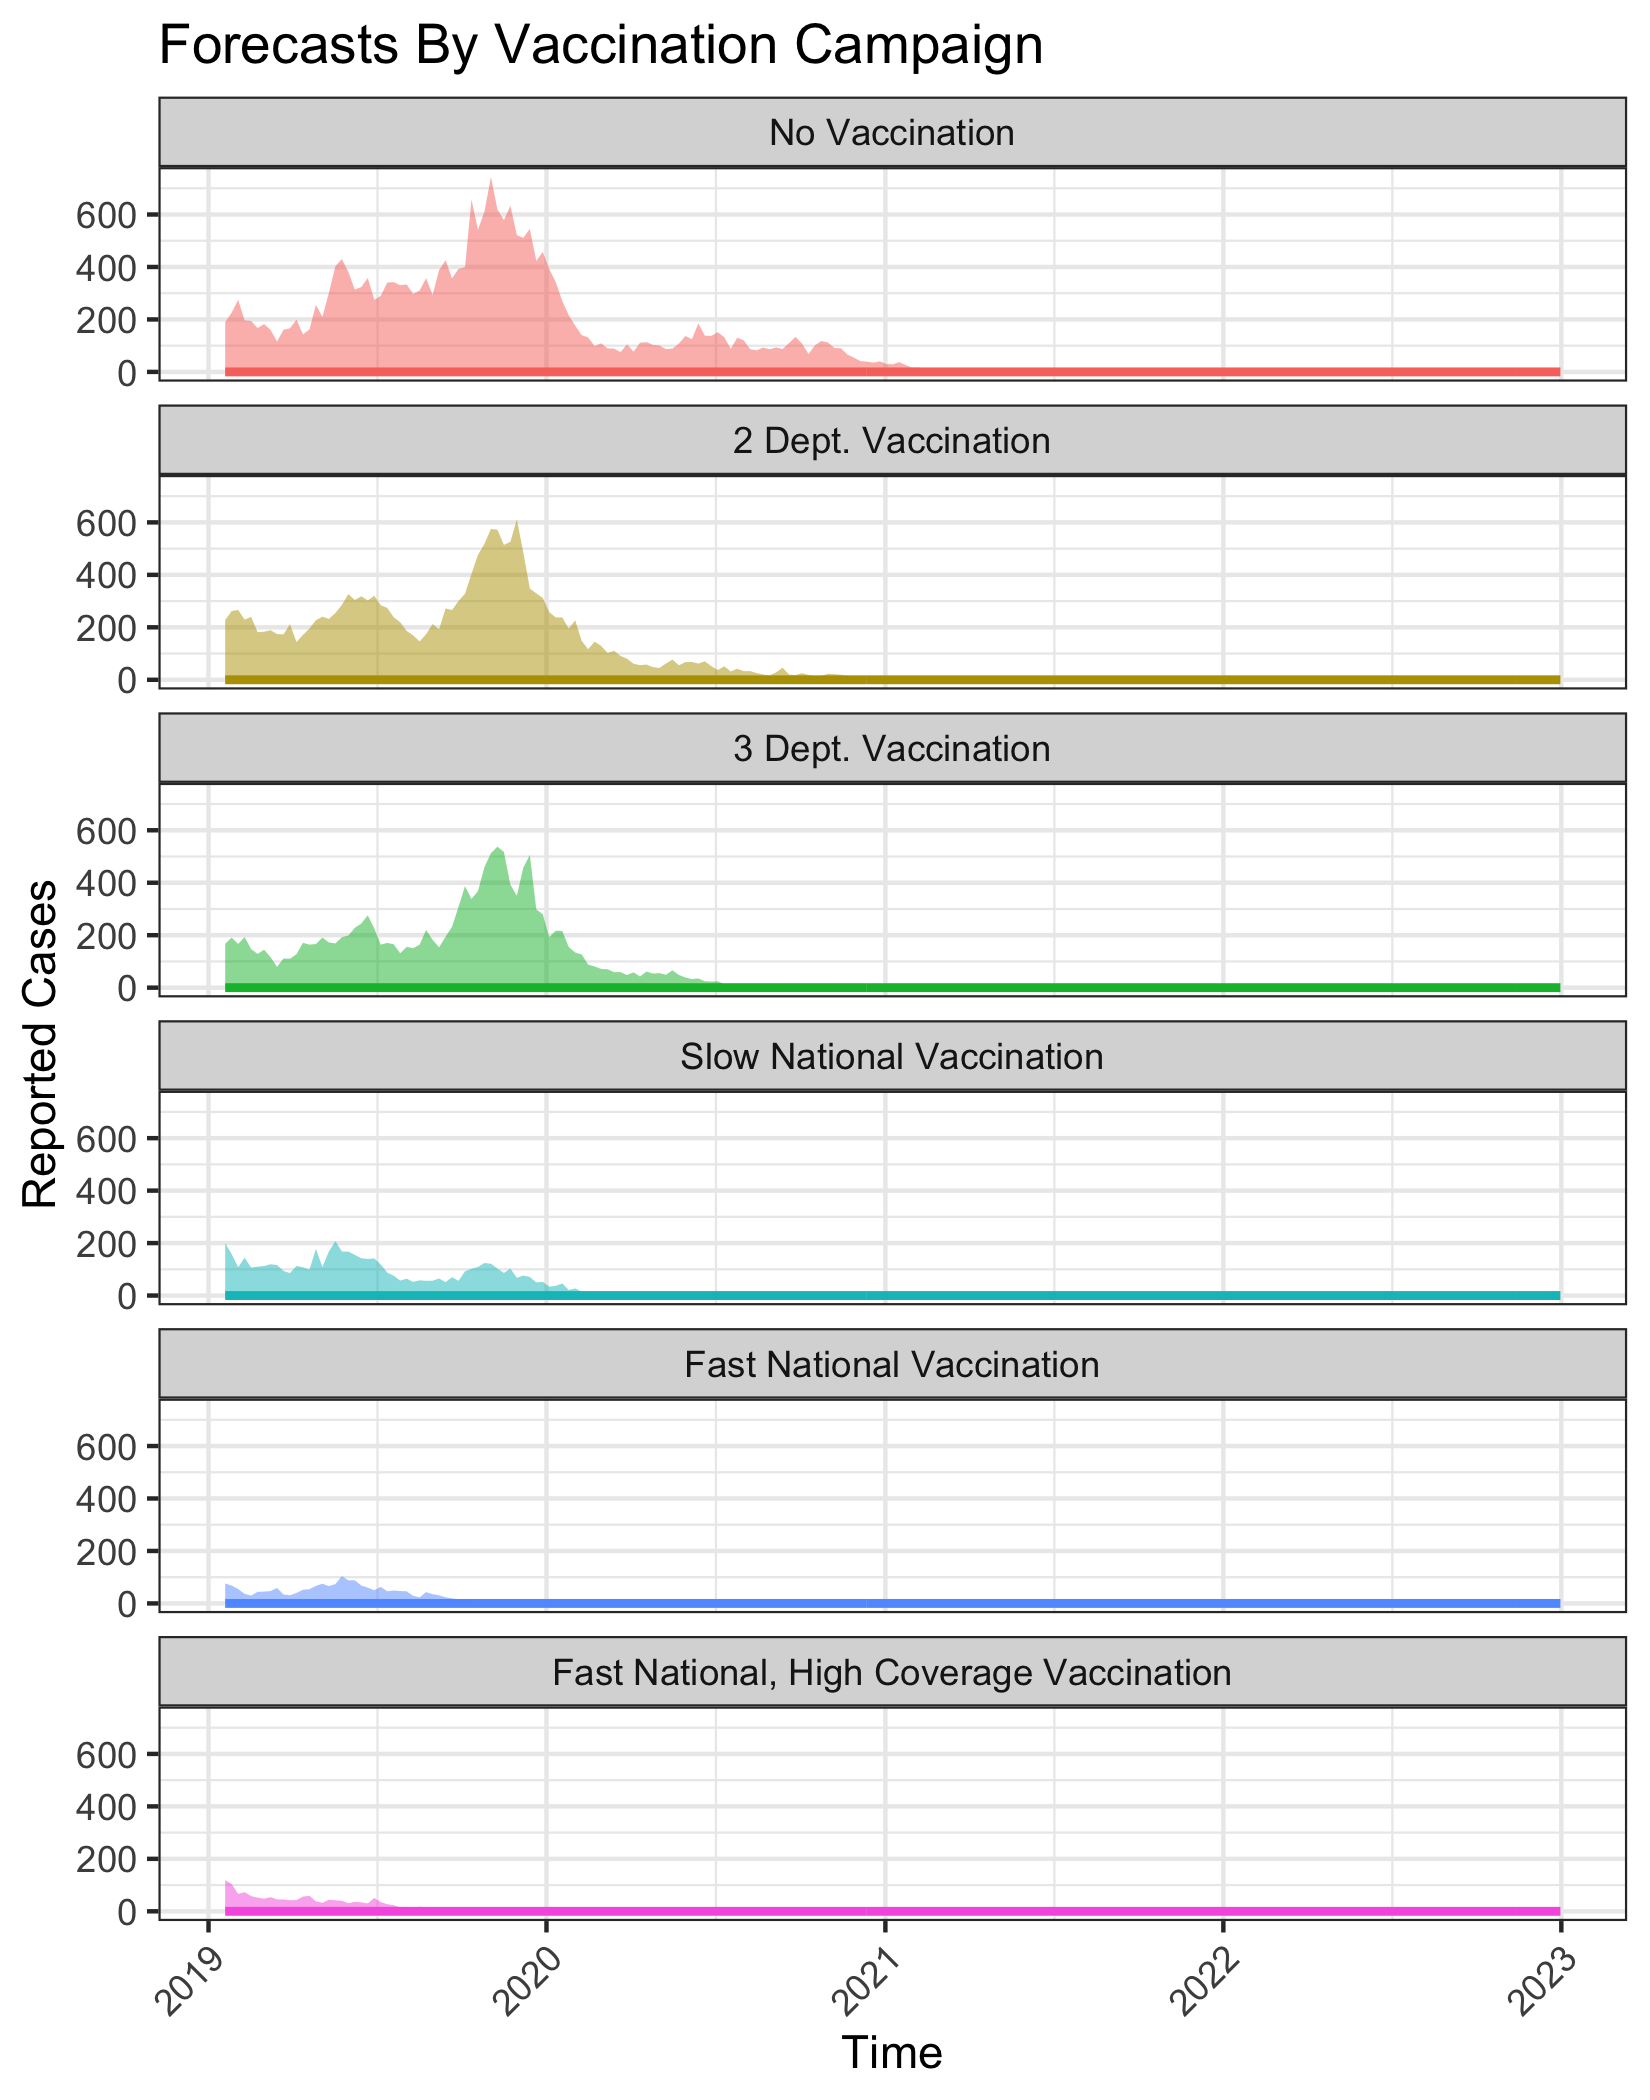
\includegraphics[width=150mm]{fc_plot.png}
  \caption{Forecast reported cases by vaccination campaign. Solid line indicates the median number of reported cases from the simulations across sets of parameters. Ribbon indicates the 2.5th and 97.5th percentiles for the simulated reported cases. Note that the plot shows forecasts until 2023 while the forecasting was conducted for a ten-year period extending until 2030. Reemergence did not occur in any campaign.}
  \label{fig:A2}
\end{figure}

\begin{figure}[H]
  \centering
  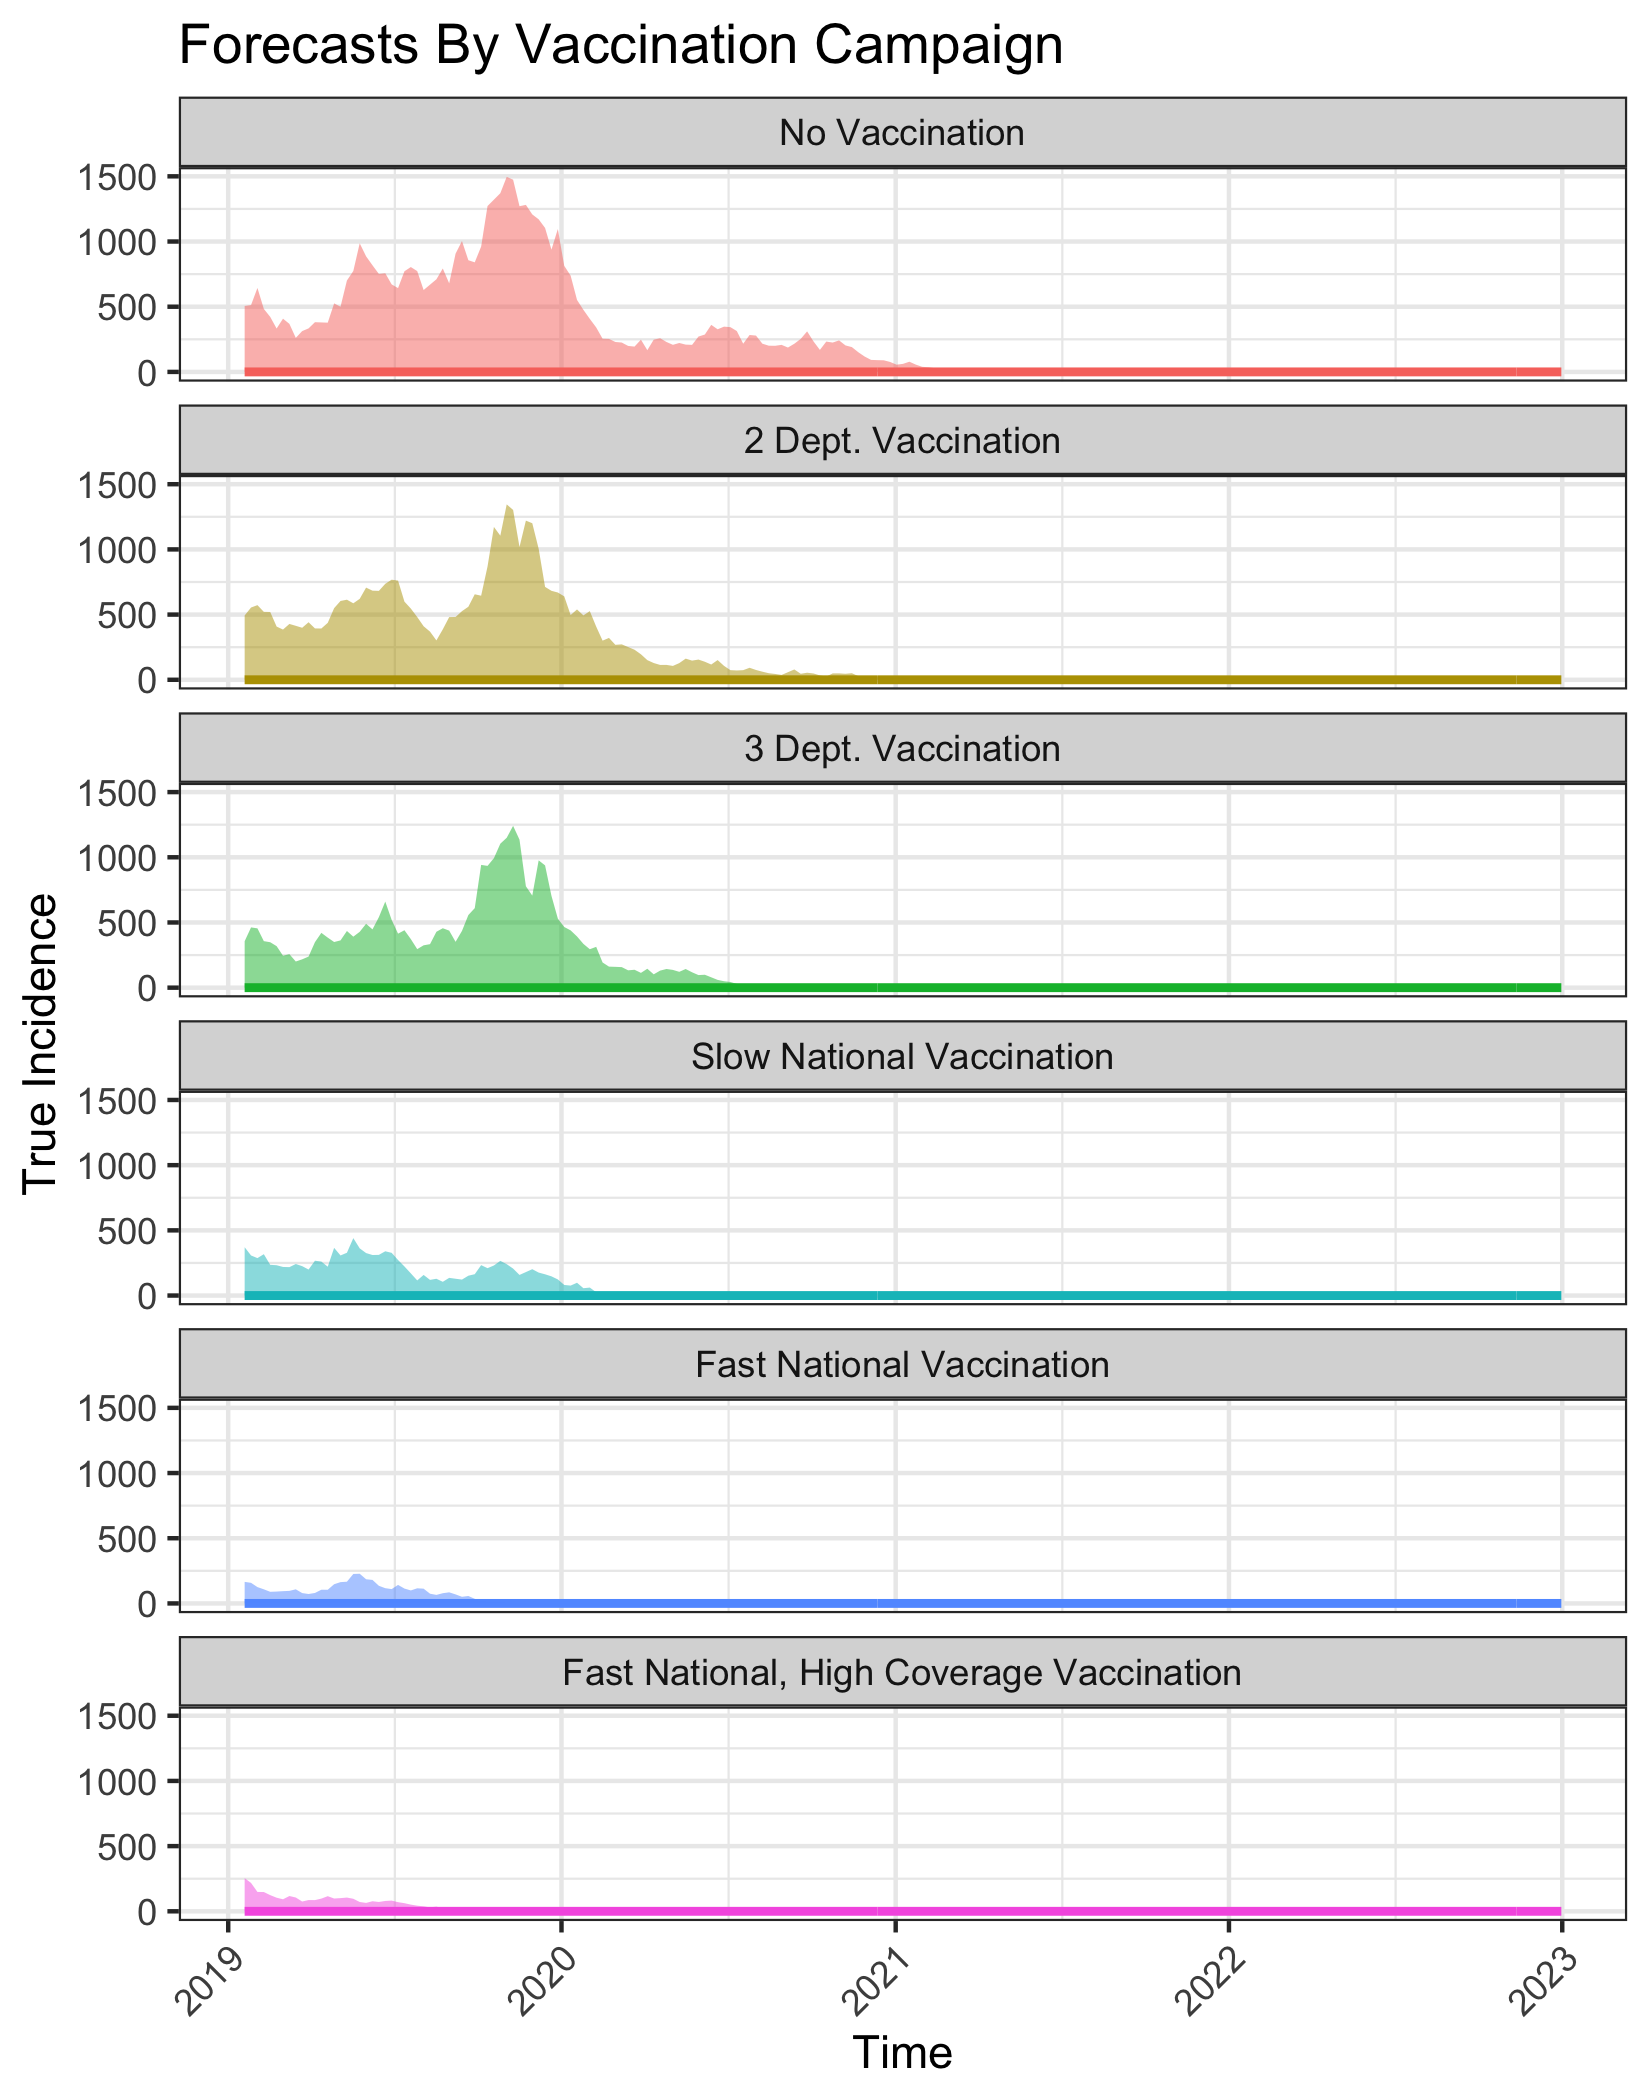
\includegraphics[width=150mm]{incid_plot.png}
  \caption{Forecast true incidence by vaccination campaign. Solid line indicates the median number of reported cases from the simulations across sets of parameters. Ribbon indicates the 2.5th and 97.5th percentiles for the simulated incidence. Note that the plot shows forecasts until 2023 while the forecasting was conducted for a ten-year period extending until 2030. Reemergence did not occur in any campaign.}
  \label{fig:A3}
\end{figure}

\begin{figure}[H]
  \centering
  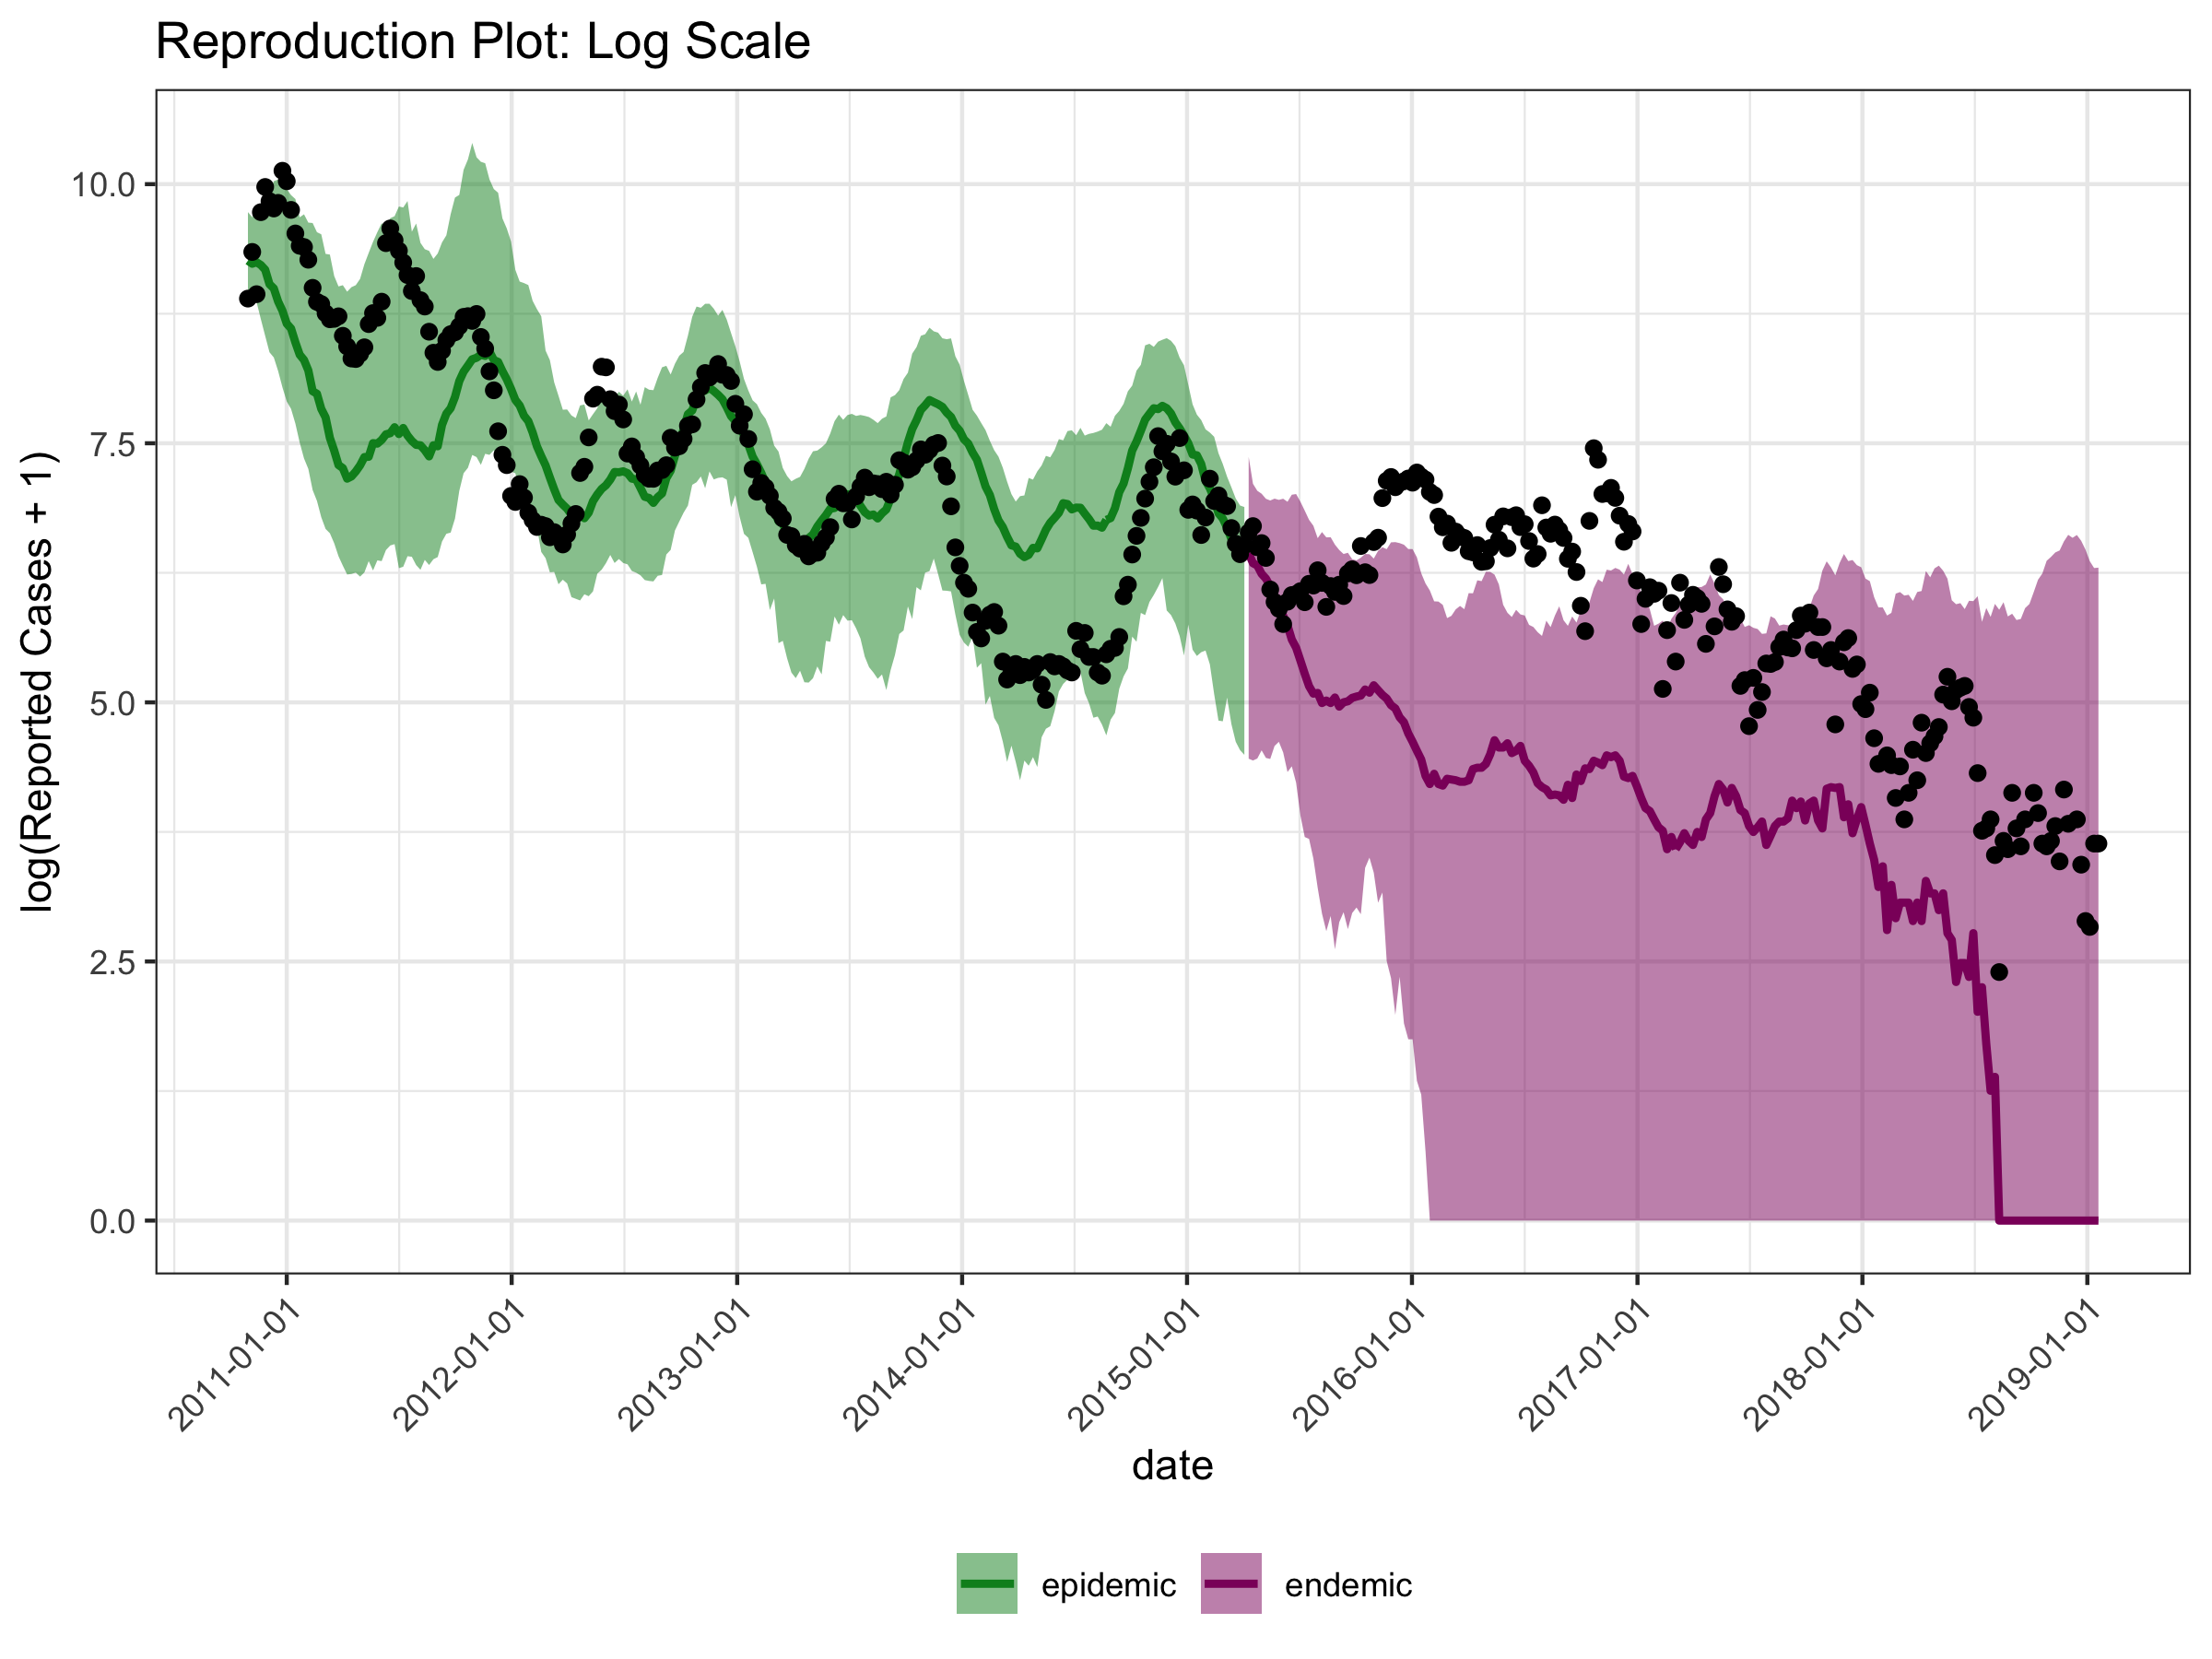
\includegraphics[width=150mm]{reprod_plot_log.png}
  \caption{Plot of original model simulations on the log scale. Solid line indicates the median simulated reported cases across parameter sets. Ribbon indicates the 2.5th and 97.5th percentiles for the simulated reported cases.}
  \label{fig:A4}
\end{figure}

\begin{figure}[H]
  \centering
  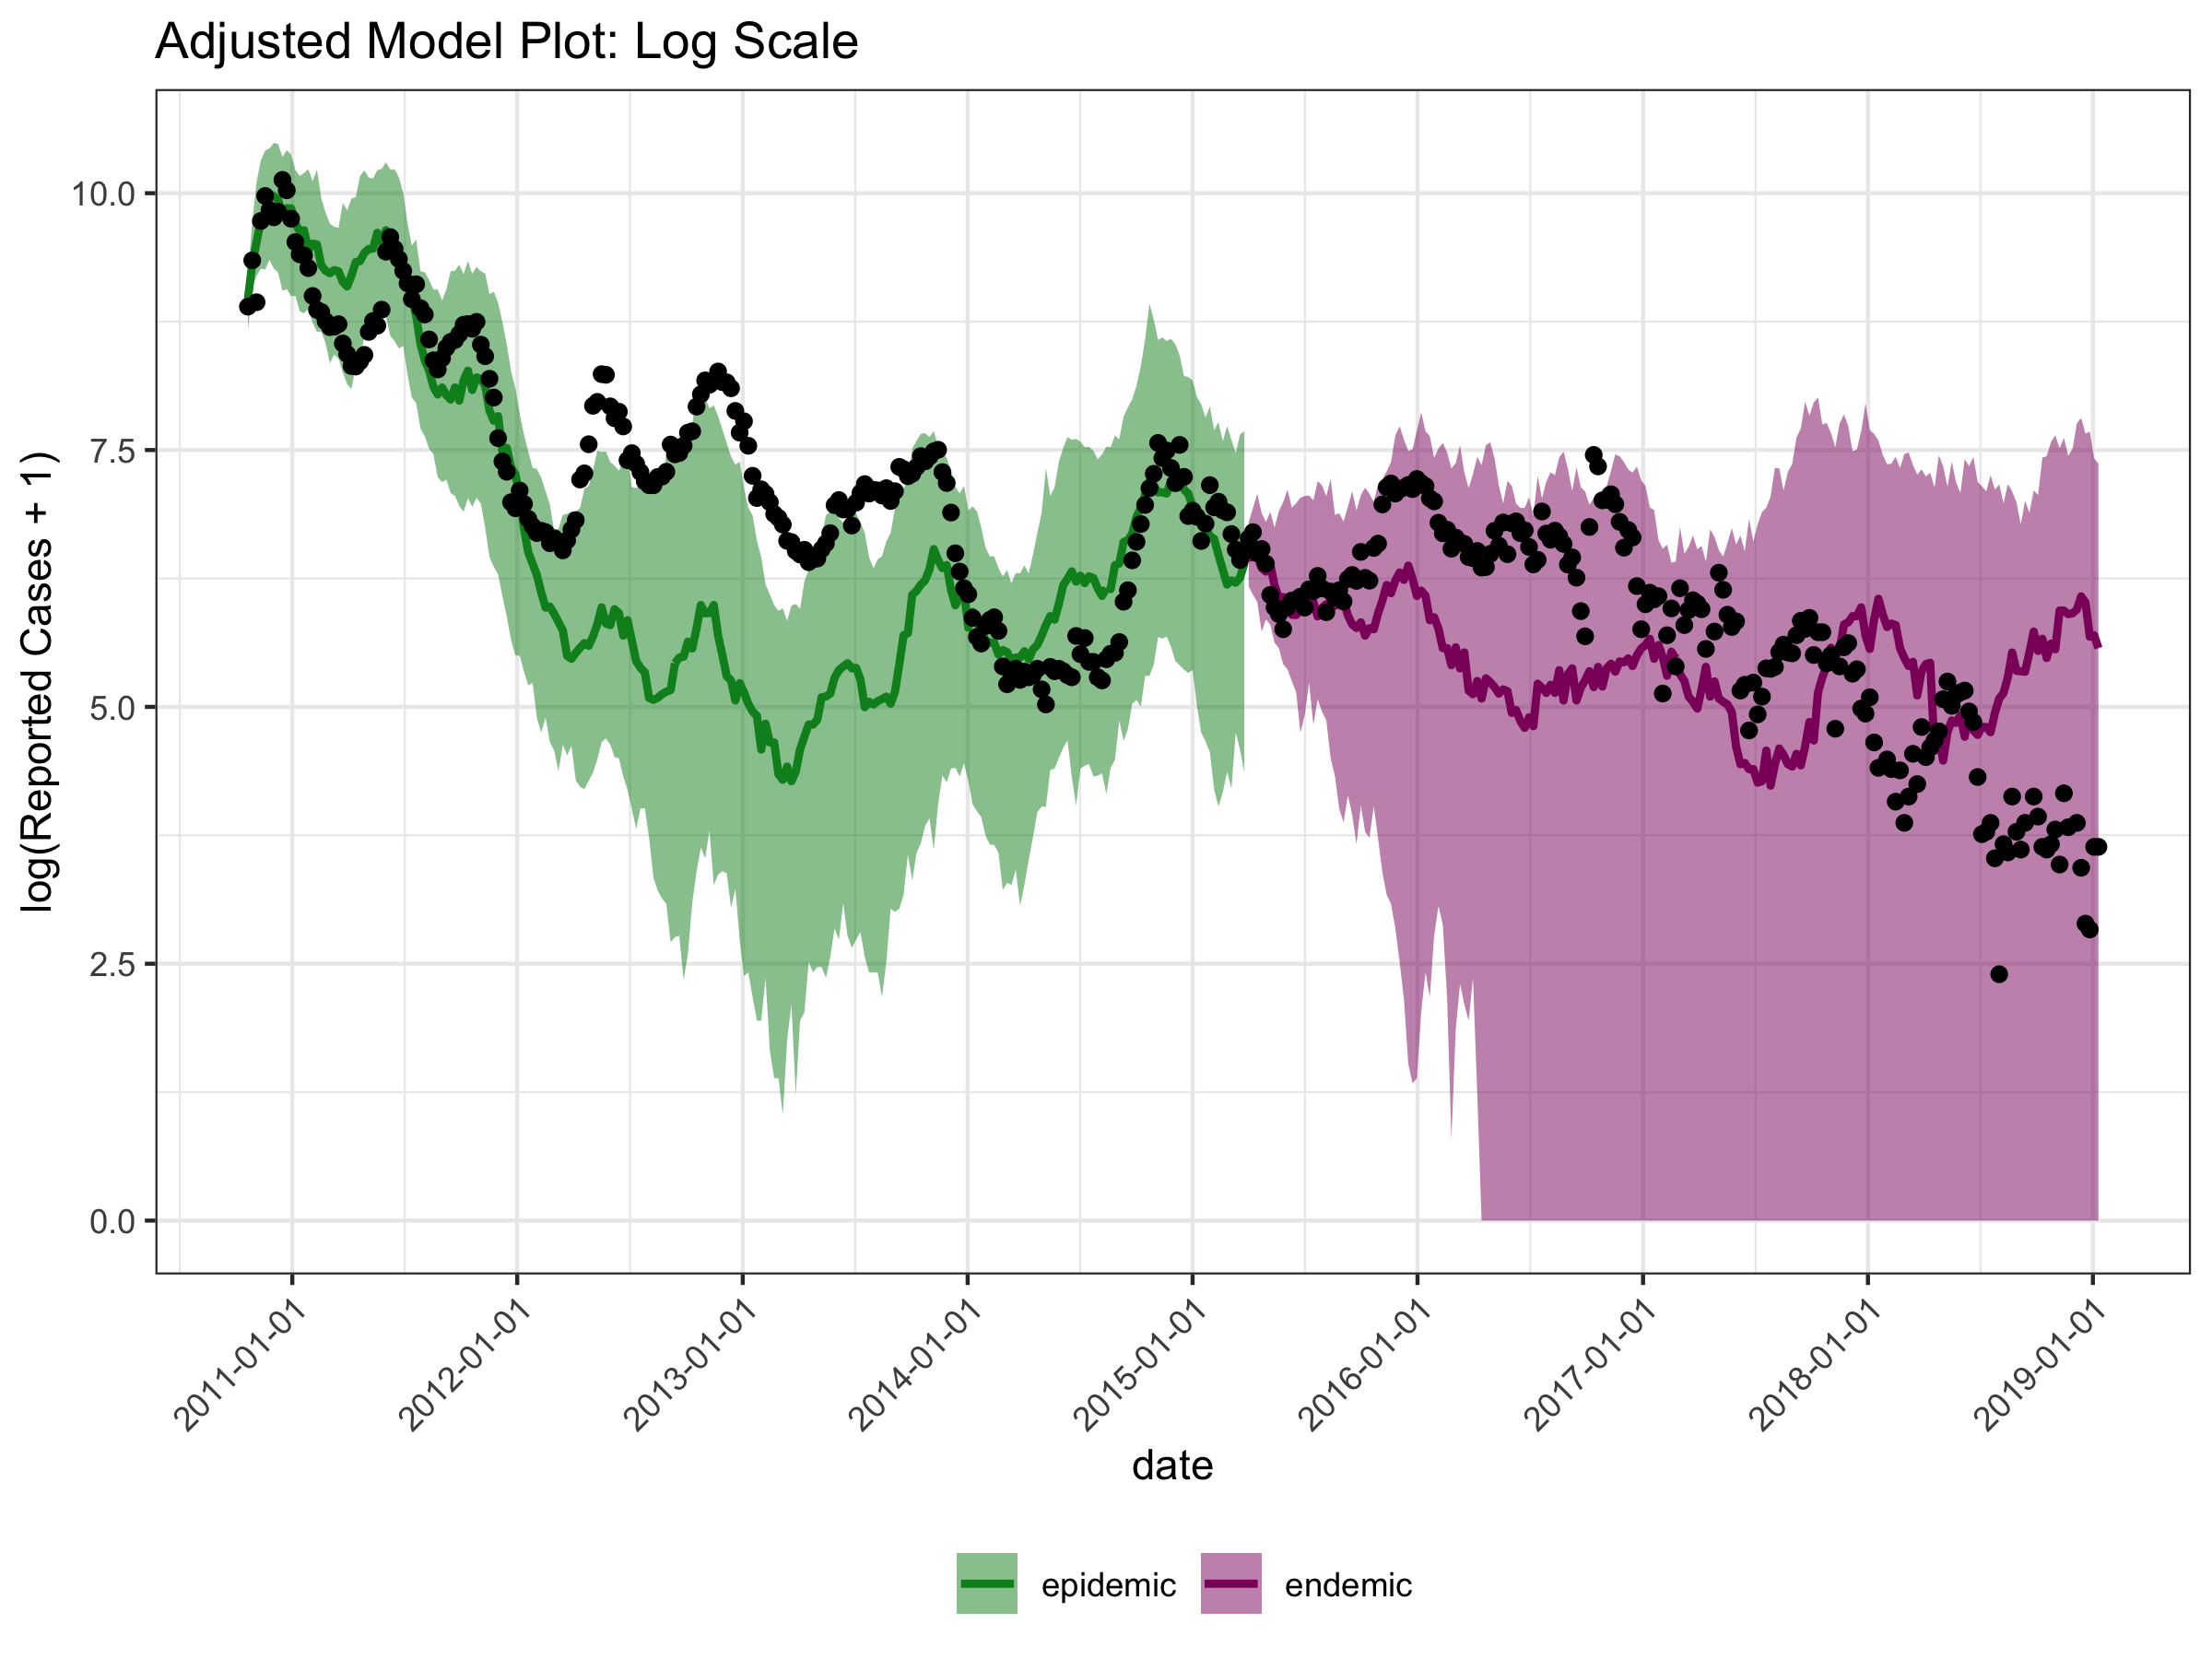
\includegraphics[width=150mm]{mle_plot_adj_log.png}
  \caption{Plot of model simulations on the log scale with overdispersion in the latent process using the parameter MLEs. Solid line indicates the median simulated reported cases across parameter sets. Ribbon indicates the 2.5th and 97.5th percentiles for the simulated reported cases.}
  \label{fig:A5}
\end{figure}

\begin{figure}[H]
  \centering
  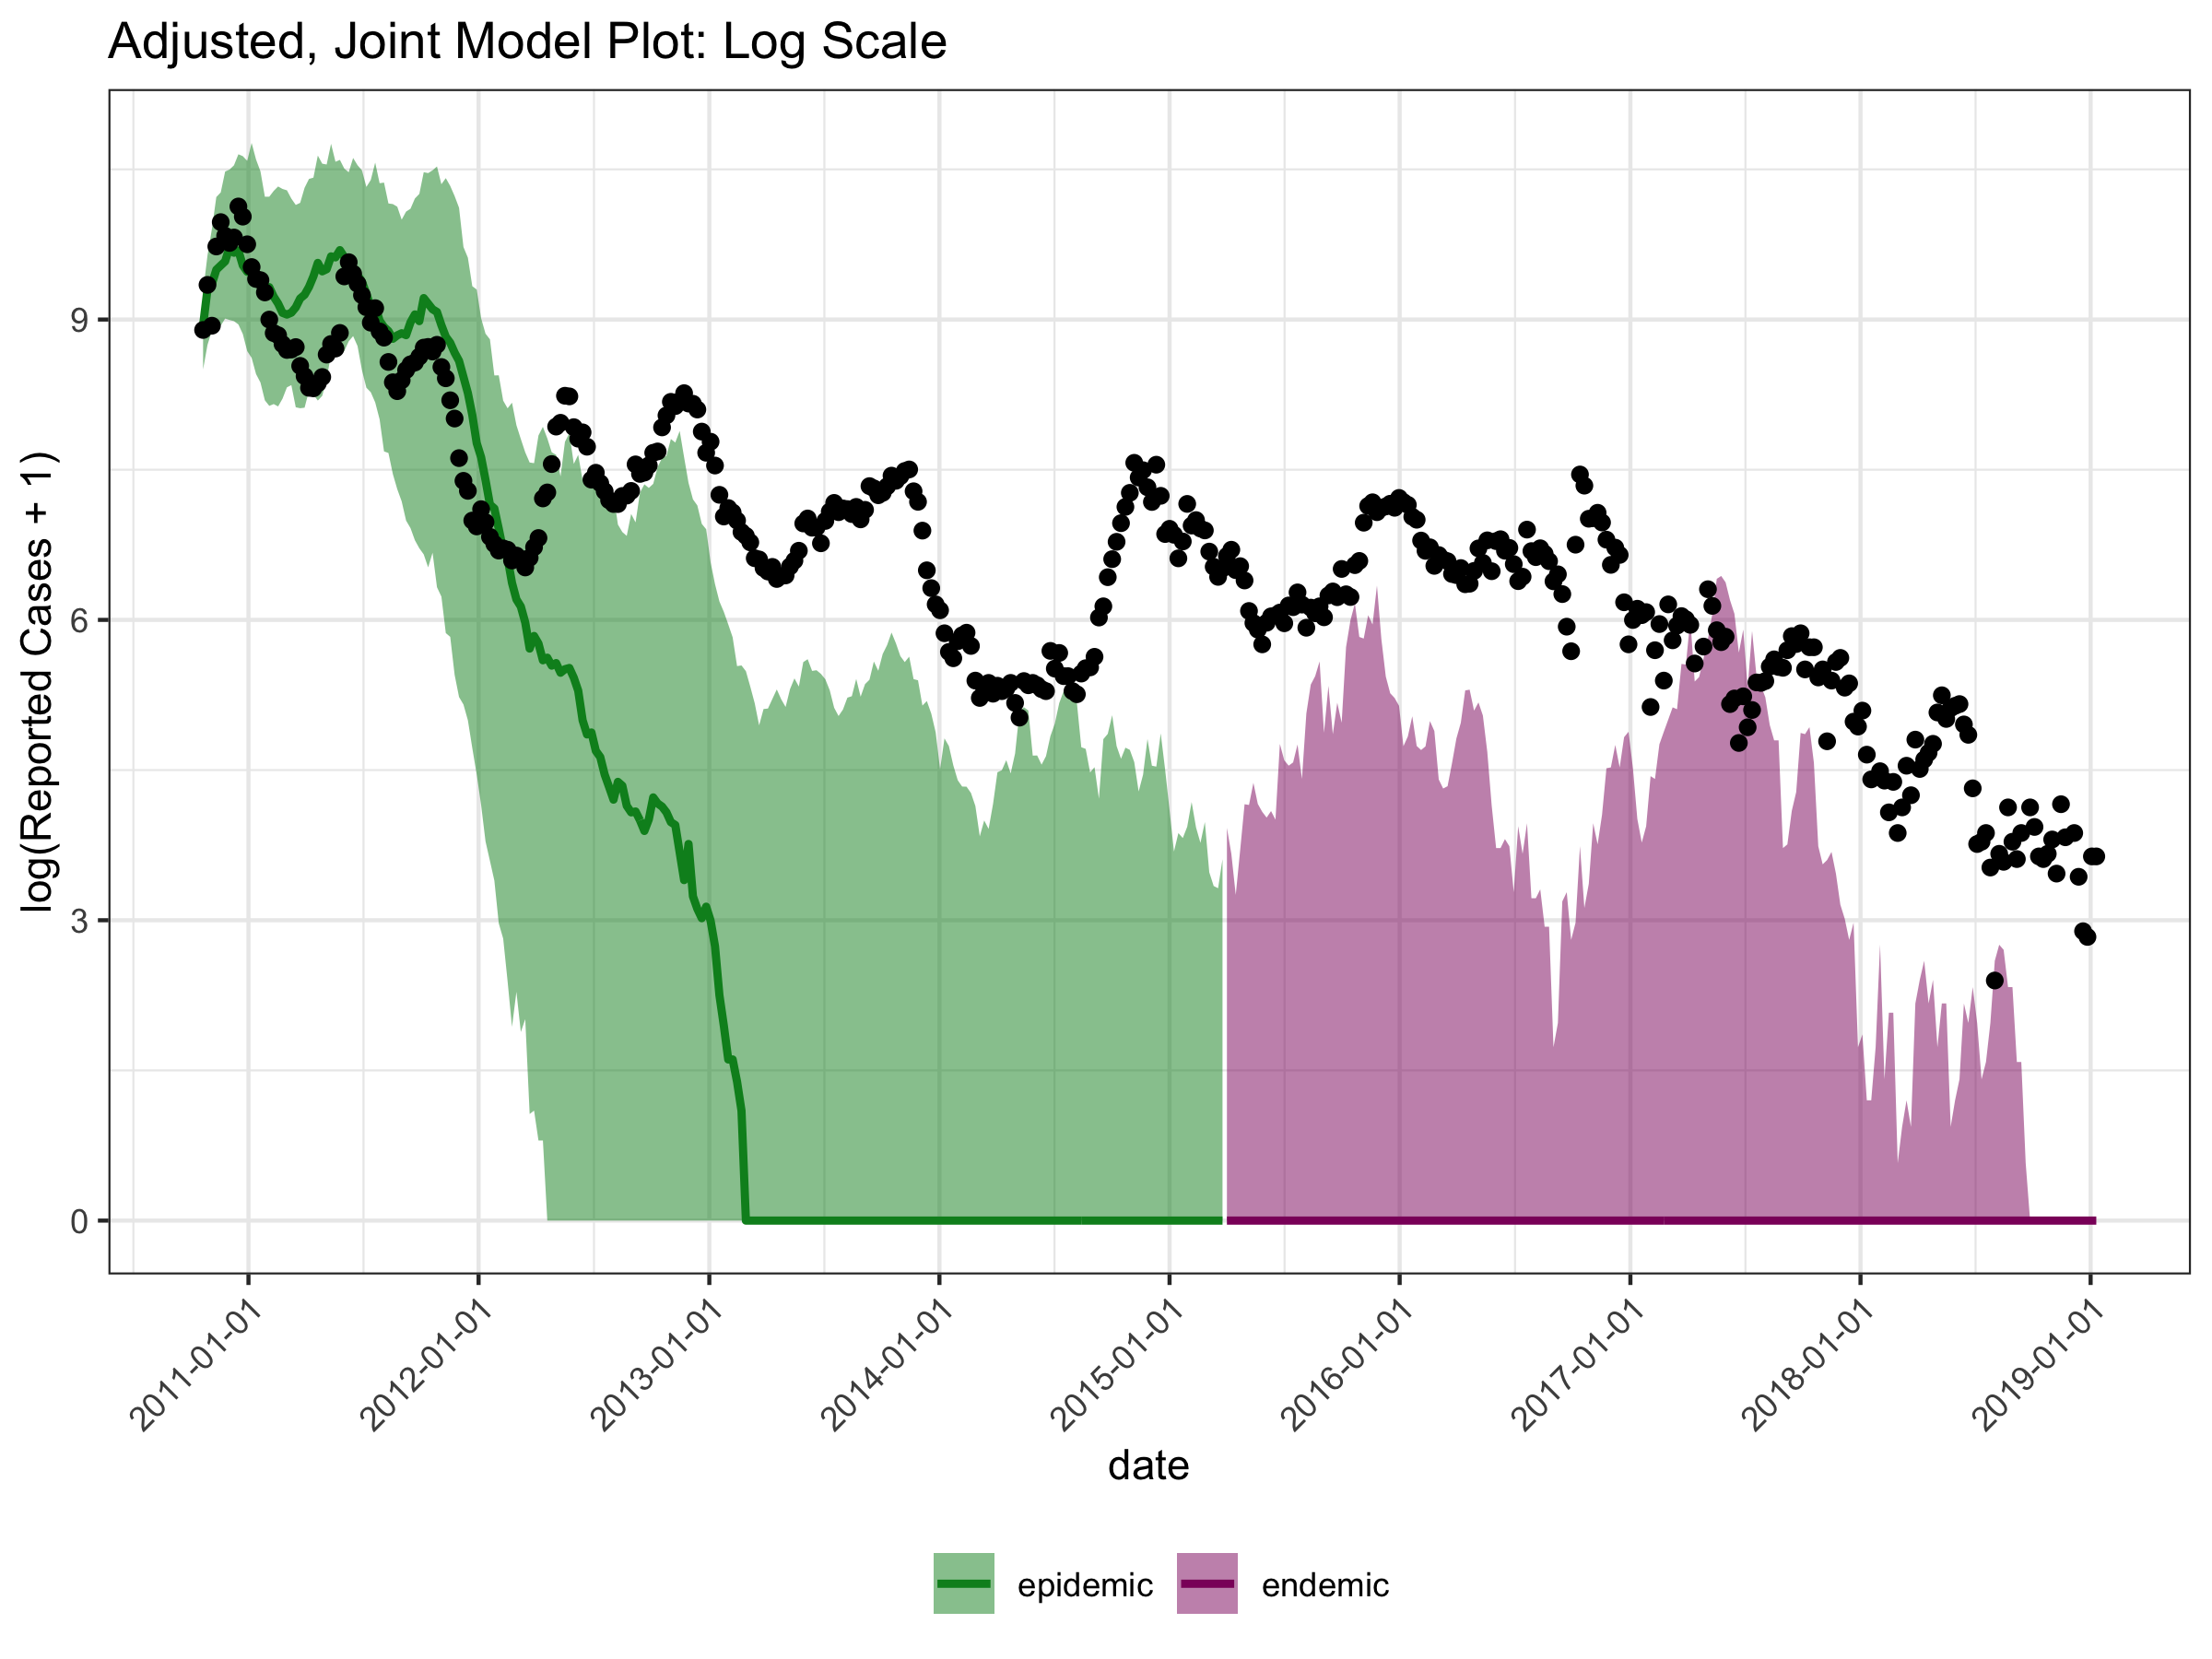
\includegraphics[width=150mm]{mle_plot_joint_log.png}
  \caption{Plot of simulations from the jointly estimated model on the log scale with additional overdispersion in the latent process using the maximum likelihood estimates of the model parameters. Solid line indicates the median number of reported cases from simulations. Ribbon indicates the 2.5th and 97.5th percentiles for the simulated reported cases.}
  \label{fig:A6}
\end{figure}

\newpage

\bibliography{bib-thesis}

\end{document}


